% ============================================================
%  第十二章 无序系统（§1–§8 + 章末参考文献）
%  底本：高等教育出版社《固体理论》第二版；原书印刷页 486–532
%  （PDF 页 = 印刷页 + 20）
%  公式编号自检：§1 (12.1.1)–(12.1.16)（(12.1.2a/b/c) 为原书自带
%    二级编号，用 subequations 环境照录，与 ch06/ch07 体例一致）；
%    §2 (12.2.1)–(12.2.35)；§3 (12.3.1)–(12.3.29)；
%    §4 (12.4.1)–(12.4.26)；§5 (12.5.1)–(12.5.41)；
%    §6 (12.6.1)–(12.6.19)；§7 (12.7.1)–(12.7.30)
%    （(12.7.13a–d) 为原书自带二级编号，subequations 照录）；
%    §8 (12.8.1)–(12.8.22)。全章自动编号 223 个，无缺号
%    （任务单 tags=217 系 (12.2.24) tag 残作"(2.2.24)"、(12.2.35)
%    残作"(.35)"、(12.3.18)(12.7.21) 编号嵌于式内、(12.3.25)
%    (12.3.26) 编号被图 12.2 挤出为游离正文、(12.6.14) OCR 丢号
%    未计入所致）。
%
%  任务单所列"缺号"逐条对照原书页面判定（均非原书跳号）：
%    (12.2.24) OCR tag 残作"(2.2.24)"，原书 p493 在号；
%    (12.2.35) OCR tag 残作"(.35)"，原书 p494 在号（三行块，
%              编号在末行右端）；
%    (12.3.18) 编号嵌于式内（p497），已归还本式；
%    (12.3.25)(12.3.26) 原书 p498 此二式与图 12.2 左右并排，
%              编号被 OCR 挤成游离正文，已归位（先式后图）；
%    (12.6.14) OCR 丢号留式，原书 p515 在号（三行块末行编号）；
%    (12.7.21) 编号嵌于式内（p521），已归还本式。
%
%  已修正的 OCR/原书错误（除全角句点转"."、删 ~ 间隔符、收紧
%  \mathrm{d}、拆开行内公式与中文等常规项外）：
%  1. 原书 p495 (12.3.3) 印作 Ĥ=K̂(ω)+[H−K(ω)]^{-1}，指数 −1 为
%     原书排印衍文（本式为哈密顿量划分，下文明言"(H−K̂)取为
%     扰动项"，且 (12.3.4) 由此式直接导出），已删。
%  2. 原书 p508 (12.5.23) 第二行末因子印作 G_{l''l'}(E)，按代入
%     (12.5.21) 于 (12.5.22) 的推导应为 G_{l''l}(E)（与同系列
%     (12.5.25) 末因子 V_{l''l} 一致），已更正。
%  3. §1 "相距任意正格矢的两个原子"按 p486 补回"$l$"；
%     "可取 V_i=2Z IJIS 及近邻 W_ij=(−2 IJIS)"按 p488 复原为
%     V_i=2Z|J|S、W_ij=(−2|J|S)；"费密算子C与C代替"按 p488 复原
%     为"费密算子 C_i 与 C_i^+ 代替"。
%  4. (12.1.9) 整块 OCR 乱码按 p489 复原为
%     Σ_l{(ω−V_i)δ_il−W_il}G(l,j;ω)=δ_ij (i,j=1,…,N)；
%     (12.1.7) 后对易式按原书补回 a_j^+（[a_i,a_j^+]_±=δ_ij）。
%  5. §2.1 "散射效应却是可以严格计算的"OCR"可 j^μ 格计算"按
%     p490 复原；"直至 V̂ 的无穷阶"按原书补回 $\hat V$（p490）。
%  6. (12.2.4)(12.2.12)(12.2.16)(12.2.17)(12.2.24)(12.2.25)
%     (12.2.35) 等多行块 OCR 乱码按 p490–494 复原；求和条件
%     j(j≠i)、l(l≠j,≠i) 等照原书。
%  7. §3 (12.3.18) 整块 OCR 乱码按 p497 复原；(12.3.25)(12.3.26)
%     游离编号归位（见上）。
%  8. §4 (12.4.2)(12.4.3) 中 OCR \hat\varepsilon_i 按原书统一为
%     ξ_i；(12.4.13) 三段等式（含 2×2 逆矩阵分子）按 p502 复原；
%     (12.4.18) OCR"F_f(ω)"按 p503 复原为 F_ff(ω)；"分别对应于
%     取 ξ_i=1 和 0"、"由此可写出有效介质的平均场哈密顿量"
%     等 OCR 错乱句按 p501–502 复原。
%  9. §5 (12.5.16)(12.5.19)(12.5.21)(12.5.23)(12.5.25) 求和哑标
%     按原书 l''(l''≠l)、l''(l''≠l,l') 复原（OCR 误作 l'）；
%     (12.5.23) 整块按 p508 复原；(12.5.38) 按 p510 复原。
% 10. 原书两处脚注 OCR 漏失，按页脚补录：p507 脚注①（无限大
%     样品的热力学极限）、p509 脚注①（自回避路径）。
% 11. §6 (12.6.14) 三行式补号（原书在号）；"这里 R̄ 存在一个特征
%     温度 T_0，它表示当 R̄=R_0 时的温度"OCR 错乱按 p516 复原；
%     W_0 OCR 误作 Ψ_0 处按 p514–515 统一为 W_0。
% 12. §7 (12.7.2) OCR 分数乱码按 p517 复原为 (πħ/e²)(R/T)；
%     (12.7.21) 三行角平均积分按 p521 复原（末两项相同故为零，
%     照原书）；(12.7.9) 后文 dp/dE=1/v 的 OCR 乱码按 p518–519
%     复原；"当 d=1 时即使 L→0 也将得到一维横截面 A_1=1"按
%     p518 复原。
% 13. §8 (12.8.1) OCR 丢指数，按 p525 补 [N(E_F)L^d]^{-1}；
%     (12.8.5) 第二行 ln(g(L)/g_d)=−2αL 按 p526 复原；
%     (12.8.16) 幂指数 ν 与因子 g(L_0)/g(L) 按 p529 复原；
%     (12.8.22) OCR"\gimel"按 p531 复原为 β(g)；OCR"两级限"
%     按 p526 改"两极限"。
% 14. 超宽行修复（改断行，未改文字）：§3.3"又因为(1/N)Tr(P̂)=ℱ(ω)=…"与 §4.4 矩形/赫伯德型态密度两句的长行内公式按可断行单位拆分；§6"对于d维(d=1,2,3)系统"括号转全角；上述两段及§4.4 末段以局部 {\sloppy} 组消除 Overfull。
% 15. 图 12.1 位置：原书图占 p507 上半页，正文句"此外，含有高
%     浓度位错的固体，取向无规的微晶系统都属拓扑无序类"被图
%     隔断，重排本按文意连排后置图。
% 16. 文献[4][5]中文条目 OCR 缺空格/粘连按 p531 复原；西文条目
%     [11]"Economon"、[14]"Abrahans""Ramakrisbnan"、[19] 年份
%     卷号、[23]"1995.25"、[28] 卷号 42 等原书如此，未改。
%  插图：图 12.1–12.9 共 9 幅均为占位图（figures/fig12-N.pdf）；
%    图 12.1 含子图说明 (a)(b)(c)、图 12.6 含 (a)(b)，图 12.3
%    原书无图注文字（仅"图 12.3"），均照原书。
%  遗留问题：
%  · (12.5.40) 洛仑兹型分布原书分子印作 ZV（归一化的洛仑兹分布
%    应为 Γ/π 型），OCR 与原书一致，照录未改；
%  · §2.4 类似地一句原书印"x⩽1 的高浓度区域"（语义应为 x≈1），
%    照录未改；
%  · §8.4 "半导工艺"疑为"半导体工艺"衍漏（p530），照录未改；
%  · §4.2 "E_f−μ=k_BT_L 为小量"之 T_L 沿用原书记号（p502）；
%  · 文献[28] 卷号 42 与文献[14] 相同，疑为 79 之误，照原书。
% ============================================================
\chapter{无序系统}

\section{无序模型}

\subsection*{1. 无序的分类}

无序是相对于有序定义的，在固体系统中无序是指相对于完整晶体中原子排列的高度有序状态的偏离.完整晶体的特点是原子排列具有严格的周期重复性，可以用点阵描述理想晶体的结构特征，在这里不仅每个原子周围原子的排列有一定的规律，而且相距任意正格矢 $\boldsymbol{l}$ 的两个原子其周围的环境相同，这就是严格的周期性，又称为固体结构的长程序.当系统的理想周期性被破坏时，就失去了长程序，成为无序系统.

固体物理学中的无序系统包括含杂质、缺陷的晶体，无序合金以及非晶态固体材料等.无序系统大致可分为两类：

（i）成分无序（compositional disorder）

例如由A、B两种原子组成的二元无序合金，每个原子处于一个确定的格点上，但究竟是A原子还是B原子处于某格点上则是随机的，这时晶格虽然存在，原子排列的周期性已被破坏，在晶体中的 $\boldsymbol{r}$ 点与 $\boldsymbol{r}+\boldsymbol{l}$ 点从结构上讲已不再是等效点，失去了长程有序，如图12.1(b).如果把不同取向的自旋看作为不同的“原子”，则磁无序系统也可归入这一类.成分无序又称替代式无序.

（ii）拓扑无序（topological disorder）

晶格已不存在，但原子排列并不像气体中原子那么杂乱无章，在一个原子间距范围内原子排列还保持一定的秩序（短程序）表现为配位数或原子间化学键的键长，键角等平均不变.最典型的例子是非晶态半导体的Ge和Si的结构，四面体键组成无规网格，完全失去了周期性，但键长和键与键之间夹角基本保持不变，近邻配位数则未必保持不变.当价键不饱和时可能出现悬挂键（dangling bonds），这时配位数就发生了变化，图12.1(c)代表同时形成了悬挂键的拓扑无序系统.此外，含有高浓度位错的固体，取向无规的微晶系统都属拓扑无序类.

\begin{center}
\begin{minipage}{9.5cm}
\centering
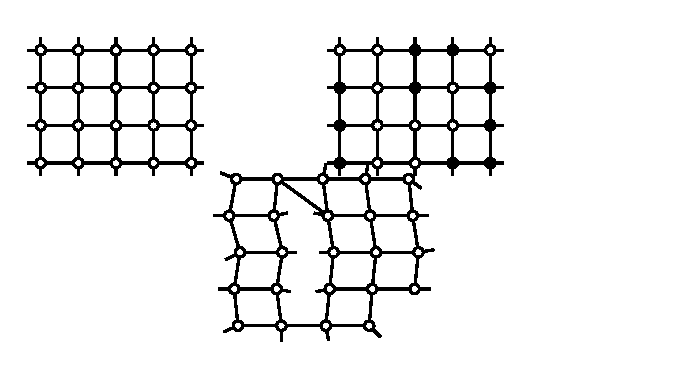
\includegraphics[width=9.5cm]{fig12-1.pdf}\\[0.3em]
{\small (a) 有序晶格\qquad\qquad (b) 成分无序系统}\\[0.2em]
{\small (c) 拓扑无序系统}\\[0.2em]
{\small 图 12.1}
\end{minipage}
\end{center}

\subsection*{2. 无序系统的模型哈密顿量}

米泽（Yonezawa）\textsuperscript{[1]}将描述固体中电子、声子和自旋波量子等各类独立准粒子系统的H用一个模型哈密顿量统一表示
\begin{equation}
  H=\sum_{i}V_{i}a_{i}^{+}a_{i}+\sum_{i\neq j}W_{ij}a_{i}^{+}a_{j}
\end{equation}
其中 $a_{i}^{+}$（$a_{i}$）是i格点上的准粒子产生（消灭）算符，$V_{i}$ 为准粒子在i格点的能量，$W_{ij}$ 描述准粒子在i与j格点之间转移的跃迁矩阵元.在此基础上，若将对角元 $V_{i}$ 取为无规变量，而 $W_{ij}$ 仍具有平移对称性，它只是 $(\boldsymbol{R}_{i}-\boldsymbol{R}_{j})$ 的函数，这时H属于对角无序系统.反之，若将 $V_{i}$ 当作与格点位置无关的常数，而取 $W_{ij}$ 与i和j格点位置以及格点上原子类型都有关的无规变量时，H将描述非对角无序系统.当 $V_{i}$ 与 $W_{ij}$ 都是无规变量时，将涉及既含对角无序，又有非对角无序的复杂无序系统.

选取式(12.1.1)统一表示H的理由来源于完整的有序晶格情形.因为当系统为有序时，H中的 $V_{i}$ 与 $W_{ij}$ 均具有平移对称性，表现为 $V_{i}=$ 常数和 $W_{ij}=W_{ij}\left(\boldsymbol{R}_{i}-\boldsymbol{R}_{j}\right)$.对于能带电子系统，当只考虑最近邻跃迁时可取 $V_{i}=\varepsilon\left(0\right)$ 及最近邻的 $W_{ij}=-J$，再将 $a_{i}$ 与 $a_{i}^{+}$ 用不计自旋标σ的费密算子 $C_{i}$ 与 $C_{i}^{+}$ 代替，上式立即简化为有序晶格中的紧束缚近似能量哈密顿量式(8.10.19).对于铁磁自旋波量子所组成的独立准粒子系统，$a_{i}$ 与 $a_{i}^{+}$ 应理解为描述自旋偏离的玻色算符，若再取 $V_{i}=2Z|J|S$ 及近邻 $W_{ij}=\left(-2|J|S\right)$，则描述有序铁磁系统的低激发态哈密顿量式(3.3.19)也可采用此模型哈密顿量.对于声子和夫伦克耳激子系统，情况也是相似的.因此，固体中各类独立元激发（准粒子）系统均可以概括为一个具有共同数学结构的模型哈密顿量，式(12.1.1).若在这一表示式的模型参数 $V_{i}$ 与 $W_{ij}$ 中引入表征无序的无规变量，H就成为描述无序系统（特别是成分无序系统）的统一哈密顿量.

我们首先讨论对角无序系统
\begin{subequations}
\begin{equation}
  H=H_{0}+H_{1}
\end{equation}
其中的有序项为
\begin{equation}
  H_{0}=\sum_{i\neq j}W_{ij}a_{i}^{+}a_{j}
\end{equation}
无序项则由
\begin{equation}
  H_{1}=\sum_{i}V_{i}a_{i}^{+}a_{i}
\end{equation}
\end{subequations}
表示，其中的 $V_{i}$ 是随机变化的.在二元无序合金 $\mathrm{A}_{x}\mathrm{B}_{1-x}$ 中，任一格点上可以被A或B原子占据的概率分别为x和(1−x)，因此i格点上 $V_{i}$ 的取值应根据概率分布
\begin{equation}
  P\left(V_{i}\right)=x\delta\left(V_{i}-V_{\mathrm{A}}\right)+\left(1-x\right)\delta\left(V_{i}-V_{\mathrm{B}}\right)
\end{equation}
决定，它既可能取 $V_{\mathrm{A}}$ 值，也可能取 $V_{\mathrm{B}}$，其中x为合金中A元素的浓度.有序项经傅里叶变换
\begin{equation*}
  W_{ij}=\frac{1}{N}\sum_{k}\varepsilon_{k}
  \mathrm{e}^{\mathrm{i}\boldsymbol{k}\cdot\left(\boldsymbol{R}_{i}-\boldsymbol{R}_{j}\right)}
\end{equation*}
可写成准粒子的能带项
\begin{equation}
  H_{0}=\sum_{k}\varepsilon_{k}a_{k}^{+}a_{k}
\end{equation}
其中 $\varepsilon_{k}$ 的能量原点取在能带的中央，相当于取 $W_{ii}=N^{-1}\sum_{k}\varepsilon_{k}=0$，这时 $W_{ij}$ 的逆变换可写为
\begin{equation}
  \varepsilon_{k}=\frac{1}{N}\sum_{i\neq j}W_{ij}
  \mathrm{e}^{-\mathrm{i}\boldsymbol{k}\cdot\left(\boldsymbol{R}_{i}-\boldsymbol{R}_{j}\right)}
\end{equation}

由于在无序系统中实际测得的物理量都是和各种无序微观相貌的平均有关的，因此对于无序系统的研究主要是计算其格林函数的无规平均
\begin{equation}
  \langle\hat{\boldsymbol{G}}\rangle=\prod_{i}\int\mathrm{d}V_{i}\,P\left(V_{i}\right)\hat{\boldsymbol{G}}
\end{equation}
为此，首先应当求出无序系统中格林函数矩阵 $\hat{\boldsymbol{G}}$ 所满足的方程.

\subsection*{3. 无序系统的格林函数方程}

定义格点格林函数
\begin{equation}
  G\left(i,j;\omega\right)\equiv\langle\langle a_{i}|a_{j}^{+}\rangle\rangle_{\omega}
\end{equation}
其中准粒子算符满足标准对易关系 $\left[a_{i},a_{j}^{+}\right]_{\pm}=\delta_{ij}$.再利用式(12.1.1)
\begin{equation}
  \left[a_{i},H\right]_{-}=V_{i}a_{i}+\sum_{l}W_{il}a_{l}
\end{equation}
并代入格林函数运动方程的通式(11.1.24)，求出格点格林函数在 $\omega$ 平面上的运动方程组
\begin{equation}
  \sum_{l}\left\{\left(\omega-V_{i}\right)\delta_{il}-W_{il}\right\}G\left(l,j;\omega\right)=\delta_{ij}
  \qquad\left(i,j=1,\cdots,N\right)
\end{equation}
这个方程组可以写成矩阵形式，定义下列（$N\times N$）矩阵
\begin{equation}
  \hat{\boldsymbol{W}}\equiv\left[W_{ij}\right],\qquad
  \hat{\boldsymbol{V}}\equiv\left[V_{i}\delta_{ij}\right],\qquad
  \hat{\boldsymbol{H}}=\hat{\boldsymbol{W}}+\hat{\boldsymbol{V}}
\end{equation}
其中 $\hat{\boldsymbol{V}}$ 为对角，而 $\hat{\boldsymbol{W}}$ 为非对角（因为取 $W_{ii}=0$）的（$N\times N$）矩阵.相应地定义格林函数矩阵
\begin{equation}
  \hat{\boldsymbol{G}}\equiv\left[G\left(i,j;\omega\right)\right]=\hat{\boldsymbol{G}}\left(\omega\right)
\end{equation}
这时可将格林函数运动方程组缩写为下列矩阵表示式：
\begin{equation}
  \left(\omega\hat{\boldsymbol{I}}-\hat{\boldsymbol{W}}-\hat{\boldsymbol{V}}\right)\hat{\boldsymbol{G}}=\hat{\boldsymbol{I}}
\end{equation}
其中 $\hat{\boldsymbol{I}}$ 代表（$N\times N$）的单位矩阵.因此，无序系统中准粒子格林函数的一般表示式为
\begin{equation}
  \hat{\boldsymbol{G}}\left(\omega\right)=\left(\omega\hat{\boldsymbol{I}}-\hat{\boldsymbol{H}}\right)^{-1}
\end{equation}
用于对角无序情形，取 $\hat{\boldsymbol{H}}_{0}=\hat{\boldsymbol{W}}$，可将 $\hat{\boldsymbol{H}}_{0}$ 的格林函数矩阵表示写成
\begin{equation}
  \hat{\boldsymbol{G}}_{0}\left(\omega\right)=\left(\omega\hat{\boldsymbol{I}}-\hat{\boldsymbol{W}}\right)^{-1}
  \ \text{或}\
  \left(\omega\hat{\boldsymbol{I}}-\hat{\boldsymbol{W}}\right)\hat{\boldsymbol{G}}_{0}=\hat{\boldsymbol{I}}
\end{equation}
从式(12.1.12)与式(12.1.14)可以导出
\begin{equation}
  \left(\omega\hat{\boldsymbol{I}}-\hat{\boldsymbol{W}}\right)
  \left(\hat{\boldsymbol{G}}-\hat{\boldsymbol{G}}_{0}\right)=\hat{\boldsymbol{V}}\hat{\boldsymbol{G}}
\end{equation}
由此求得对角无序系统中准粒子格林函数所满足的标准运动方程：
\begin{equation}
  \hat{\boldsymbol{G}}=\hat{\boldsymbol{G}}_{0}+\hat{\boldsymbol{G}}_{0}\hat{\boldsymbol{V}}\hat{\boldsymbol{G}}
\end{equation}
其中 $\hat{\boldsymbol{G}}_{0}$ 是有序系统 $\hat{\boldsymbol{H}}_{0}$ 的格林函数，它具有平移对称性.因此，在计算无序格林函数的无规平均 $\langle\hat{\boldsymbol{G}}\rangle$ 时，将涉及关联项 $\hat{\boldsymbol{V}}\hat{\boldsymbol{G}}$ 的无规平均 $\langle\hat{\boldsymbol{V}}\hat{\boldsymbol{G}}\rangle$.由于 $\hat{\boldsymbol{V}}\hat{\boldsymbol{G}}$ 可以用t矩阵表示，其无规平均 $\langle\hat{\boldsymbol{V}}\hat{\boldsymbol{G}}\rangle$ 的计算自然将涉及如何计算t矩阵的无序平均.

\section{\texorpdfstring{平均$ t $矩阵方法}{平均t矩阵方法}}

\subsection*{1. 无序系统的$ t $矩阵}

t矩阵定义为
\begin{equation}
  \hat{\boldsymbol{G}}=\hat{\boldsymbol{G}}_{0}+\hat{\boldsymbol{G}}_{0}\hat{T}\hat{\boldsymbol{G}}_{0}
\end{equation}
根据式(12.1.16)可求得 $\hat{\boldsymbol{G}}$ 的一个表示式
\begin{equation}
  \hat{\boldsymbol{G}}=\left(1-\hat{\boldsymbol{G}}_{0}\hat{\boldsymbol{V}}\right)^{-1}\hat{\boldsymbol{G}}_{0}
\end{equation}
再将上式代入式(12.1.16)求得
\begin{equation}
  \hat{\boldsymbol{G}}=\hat{\boldsymbol{G}}_{0}+\hat{\boldsymbol{G}}_{0}\hat{\boldsymbol{V}}
  \left(1-\hat{\boldsymbol{G}}_{0}\hat{\boldsymbol{V}}\right)^{-1}\hat{\boldsymbol{G}}_{0}
\end{equation}
因此无序系统的t矩阵可表示为
\begin{equation}
\begin{aligned}
  \hat{T}=\hat{T}\left(\omega\right)
  &=\hat{\boldsymbol{V}}\left(1-\hat{\boldsymbol{G}}_{0}\hat{\boldsymbol{V}}\right)^{-1}\\
  &=\hat{\boldsymbol{V}}+\hat{\boldsymbol{V}}\hat{\boldsymbol{G}}_{0}\hat{\boldsymbol{V}}
  +\hat{\boldsymbol{V}}\hat{\boldsymbol{G}}_{0}\hat{\boldsymbol{V}}\hat{\boldsymbol{G}}_{0}\hat{\boldsymbol{V}}+\cdots
\end{aligned}
\end{equation}
其中包括了对角无序 $\hat{\boldsymbol{V}}$ 所引起的相对于 $\hat{\boldsymbol{G}}_{0}$ 的所有散射，直至 $\hat{\boldsymbol{V}}$ 的无穷阶.

对 $\hat{\boldsymbol{G}}$ 取无规平均，可将式(12.2.1)表示为
\begin{equation}
  \langle\hat{\boldsymbol{G}}\rangle=\hat{\boldsymbol{G}}_{0}
  +\hat{\boldsymbol{G}}_{0}\langle\hat{T}\rangle\hat{\boldsymbol{G}}_{0}
\end{equation}
其中 $\hat{\boldsymbol{G}}_{0}$ 是有序系统的格林函数，无需平均.再定义自能
\begin{equation}
  \hat{\boldsymbol{\Sigma}}\left(\omega\right)\equiv
  \hat{\boldsymbol{G}}_{0}^{-1}-\langle\hat{\boldsymbol{G}}\rangle^{-1}
\end{equation}
又有
\begin{equation}
  \langle\hat{\boldsymbol{G}}\rangle=\hat{\boldsymbol{G}}_{0}
  +\hat{\boldsymbol{G}}_{0}\hat{\boldsymbol{\Sigma}}\left(\omega\right)\langle\hat{\boldsymbol{G}}\rangle
\end{equation}
利用式(12.2.5)—式(12.2.7)可求得自能 $\hat{\boldsymbol{\Sigma}}$ 与平均t矩阵 $\langle\hat{T}\rangle$ 的严格关系
\begin{equation}
  \hat{\boldsymbol{\Sigma}}=\left(1+\langle\hat{T}\rangle\hat{\boldsymbol{G}}_{0}\right)^{-1}\langle\hat{T}\rangle
\end{equation}
上式表明自能完全由 $\langle\hat{T}\rangle$ 决定.剩下的问题是如何计算 $\langle\hat{T}\rangle$？实际上 $\langle\hat{T}\rangle$ 不可能严格求出.但是，单个杂质相对于基体 $\hat{\boldsymbol{G}}_{0}$ 的散射效应却是可以严格计算的.为此，我们将先介绍单个原子的t矩阵.

\subsection*{2. 原子的$ t $矩阵}

为了严格计入在某一格点上单个无序杂质的多重散射效应，将 $\hat{\boldsymbol{V}}$ 分解为
\begin{equation}
  \hat{\boldsymbol{V}}\equiv\sum_{i}\hat{V}_{i}
\end{equation}
其中 $\hat{\boldsymbol{V}}$ 为（$N\times N$）对角矩阵.$\hat{V}_{i}$ 也是（$N\times N$）矩阵，但其中仅在i格点上有扰动 $V_{i}$，其它的对角元素 $(j\neq i)$ 均为零.再将式(12.2.4)改写成 $\hat{T}\left(1-\hat{\boldsymbol{G}}_{0}\hat{\boldsymbol{V}}\right)=\hat{\boldsymbol{V}}$，可得
\begin{equation}
  \hat{T}=\left(1+\hat{T}\hat{\boldsymbol{G}}_{0}\right)\hat{\boldsymbol{V}}
  =\sum_{i}\left[1+\Bigl(\sum_{j}\hat{T}_{j}\Bigr)\hat{\boldsymbol{G}}_{0}\right]\hat{V}_{i}
  =\sum_{i}\hat{T}_{i}
\end{equation}
其中 $\hat{T}_{i}$ 表示在含有多杂质的无序系统中i格点对 $\hat{T}$ 矩阵的贡献
\begin{equation}
  \hat{T}_{i}=\hat{V}_{i}+\Bigl(\sum_{j}\hat{T}_{j}\Bigr)\hat{\boldsymbol{G}}_{0}\hat{V}_{i}
  =\left(\hat{V}_{i}+\hat{T}_{i}\hat{\boldsymbol{G}}_{0}\hat{V}_{i}\right)
  +\sum_{j(j\neq i)}\hat{T}_{j}\hat{\boldsymbol{G}}_{0}\hat{V}_{i}
\end{equation}
上式中最后一项代表其它格点 $j\left(j\neq i\right)$ 的影响，而前两项则是同格点的贡献.若将来自i格点上单个原子的t矩阵定义为
\begin{equation}
\begin{aligned}
  \hat{t}_{i}&\equiv\hat{V}_{i}\left(1-\hat{\boldsymbol{G}}_{0}\hat{V}_{i}\right)^{-1}\\
  &=\hat{V}_{i}+\hat{V}_{i}\hat{\boldsymbol{G}}_{0}\hat{V}_{i}
  +\hat{V}_{i}\hat{\boldsymbol{G}}_{0}\hat{V}_{i}\hat{\boldsymbol{G}}_{0}\hat{V}_{i}+\cdots
\end{aligned}
\end{equation}
这是一个准至 $V_{i}$ 无穷阶的“部分求和”，它计入了单个原子的全部多重散射.因此，在物理上 $\hat{t}_{i}$ 描述一个波被第i个原子的完全散射，而在数学上 $\hat{t}_{i}$ 相当于略去式(12.2.11)等式右边最后一项（即略去来自 $j\neq i$ 的贡献）时所求出的近似 $\hat{T}_{i}$.至于严格的 $\hat{T}_{i}$ 应当从式(12.2.11)的下列等效表示式
\begin{equation}
  \hat{T}_{i}\left(1-\hat{\boldsymbol{G}}_{0}\hat{V}_{i}\right)
  =\hat{V}_{i}+\sum_{j(j\neq i)}\hat{T}_{j}\hat{\boldsymbol{G}}_{0}\hat{V}_{i}
\end{equation}
导出，由此求得 $\hat{T}_{i}$ 的严格公式
\begin{equation}
  \hat{T}_{i}=\hat{t}_{i}+\sum_{j(j\neq i)}\hat{T}_{j}\hat{\boldsymbol{G}}_{0}\hat{t}_{i}
\end{equation}
其中除来自i格点的贡献外，还包括了i格点以外的其它(N−1)个格点上的原子对i格点上波的散射效应.再作迭代运算，就求得整个无序系统的t矩阵
\begin{equation}
\begin{aligned}
  \hat{T}=\sum_{i}\hat{T}_{i}
  &=\sum_{i}\hat{t}_{i}+\sum_{i}\sum_{j(j\neq i)}\hat{t}_{j}\hat{\boldsymbol{G}}_{0}\hat{t}_{i}\\
  &\quad+\sum_{i}\sum_{j(j\neq i)}\sum_{l(l\neq j,\neq i)}
  \hat{t}_{l}\hat{\boldsymbol{G}}_{0}\hat{t}_{j}\hat{\boldsymbol{G}}_{0}\hat{t}_{i}+\cdots
\end{aligned}
\end{equation}
显然，当计算 $\langle\hat{T}\rangle$ 时将涉及不同格点上原子t矩阵的散射关联项，如 $\langle\hat{t}_{j}\hat{\boldsymbol{G}}_{0}\hat{t}_{i}\rangle$、$\langle\hat{t}_{l}\hat{\boldsymbol{G}}_{0}\hat{t}_{j}\hat{\boldsymbol{G}}_{0}\hat{t}_{i}\rangle$ 等无穷个关联项，在原则上是无法严格求解的.人们只能求助于各种近似，其中最常用的是平均t矩阵近似（简称ATA）的单格点近似（简称SSA）.

\subsection*{3. ATA 的单格点近似}

SSA略去了不同格点间散射的关联，仅对 $\hat{T}$ 中各格点的原子t矩阵（如 $\hat{t}_{i}$、$\hat{t}_{j}$ 和 $\hat{t}_{l}$）独立取无规平均，这时SSA的ATA表示式为
\begin{equation}
\begin{aligned}
  \langle\hat{T}\rangle&=\sum_{i}\langle\hat{t}_{i}\rangle
  +\sum_{j(j\neq i)}\langle\hat{t}_{j}\rangle\hat{\boldsymbol{G}}_{0}\sum_{i}\langle\hat{t}_{i}\rangle\\
  &\quad+\sum_{l(l\neq j)}\langle\hat{t}_{l}\rangle\hat{\boldsymbol{G}}_{0}\sum_{j(j\neq i)}\langle\hat{t}_{j}\rangle
  \hat{\boldsymbol{G}}_{0}\sum_{i}\langle\hat{t}_{i}\rangle+\cdots
\end{aligned}
\end{equation}
同时可将式(12.2.14)的无规平均写成下列SSA表示式
\begin{equation}
\begin{aligned}
  \langle\hat{T}_{i}\rangle&=\langle\hat{t}_{i}\rangle
  +\sum_{j(j\neq i)}\langle\hat{T}_{j}\rangle\hat{\boldsymbol{G}}_{0}\langle\hat{t}_{i}\rangle\\
  &=\left(1+\langle\hat{T}\rangle\hat{\boldsymbol{G}}_{0}\right)\langle\hat{t}_{i}\rangle
  -\langle\hat{T}_{i}\rangle\hat{\boldsymbol{G}}_{0}\langle\hat{t}_{i}\rangle
\end{aligned}
\end{equation}
经整理，求得单格点近似下无序系统的平均t矩阵
\begin{equation}
  \langle\hat{T}\rangle=\sum_{i}\langle\hat{T}_{i}\rangle
  =\left(1+\langle\hat{T}\rangle\hat{\boldsymbol{G}}_{0}\right)\sum_{i}\langle\hat{t}_{i}\rangle
  \left(1+\hat{\boldsymbol{G}}_{0}\langle\hat{t}_{i}\rangle\right)^{-1}
\end{equation}
将上式代入自能公式(12.2.8)，又可求出SSA的自能矩阵
\begin{equation}
  \hat{\boldsymbol{\Sigma}}_{\mathrm{SSA}}=\sum_{i}\langle\hat{t}_{i}\rangle
  \left(1+\hat{\boldsymbol{G}}_{0}\langle\hat{t}_{i}\rangle\right)^{-1}
\end{equation}
和相应的格林函数矩阵
\begin{equation}
  \langle\hat{\boldsymbol{G}}\rangle_{\mathrm{SSA}}
  =\left(\hat{\boldsymbol{G}}_{0}^{-1}-\hat{\boldsymbol{\Sigma}}_{\mathrm{SSA}}\right)^{-1}
\end{equation}

现在讨论二元无序合金 $\mathrm{A}_{x}\mathrm{B}_{1-x}$ 中A与B原子的t矩阵 $\hat{t}_{\mathrm{A}(\mathrm{B})}$ 的表示式.从原子t矩阵的定义式(12.2.12)可知，$\hat{t}_{i}$ 与 $\hat{V}_{i}$ 相似只有第i个对角元 $V_{i}$ 为非零.当i格点被A（或B）原子占据时，其对角矩阵元定义为
\begin{equation}
  t_{\mathrm{A}(\mathrm{B})}\equiv\langle i|\hat{t}_{\mathrm{A}(\mathrm{B})}|i\rangle
\end{equation}
根据二元无序合金的概率分布公式(12.1.3)可求出i格点上原子t矩阵的无规平均 $\langle\hat{t}_{i}\rangle$ 的唯一非零对角元为
\begin{equation}
  xt_{\mathrm{A}}+\left(1-x\right)t_{\mathrm{B}}
\end{equation}
显然它与i无关，因此 $\Bigl\langle\sum_{i}\hat{t}_{i}\Bigr\rangle$ 是对角矩阵，并且每个对角元均相同，可写成
\begin{equation}
  \Bigl\langle\sum_{i}\hat{t}_{i}\Bigr\rangle=x\hat{t}_{\mathrm{A}}+\left(1-x\right)\hat{t}_{\mathrm{B}}
\end{equation}
其中 $\Bigl\langle\sum_{i}\hat{t}_{i}\Bigr\rangle$、$\hat{t}_{\mathrm{A}}$ 和 $\hat{t}_{\mathrm{B}}$ 都是（$N\times N$）对角矩阵.为了求出 $t_{\mathrm{A}}$ 和 $t_{\mathrm{B}}$ 的表示式，应从（$N\times N$）无规矩阵 $\sum_{i}\hat{t}_{i}$ 入手，计算其第i个对角元
\begin{equation}
\begin{aligned}
  t_{i}&=\langle i|\hat{t}_{i}|i\rangle
  =\langle i|\left(\hat{V}_{i}+\hat{V}_{i}\hat{\boldsymbol{G}}_{0}\hat{V}_{i}
  +\hat{V}_{i}\hat{\boldsymbol{G}}_{0}\hat{V}_{i}\hat{\boldsymbol{G}}_{0}\hat{V}_{i}+\cdots\right)|i\rangle\\
  &=\frac{V_{i}}{1-\langle i|\hat{\boldsymbol{G}}_{0}|i\rangle V_{i}}
  =\frac{V_{i}}{1-\left(1/N\right)\left(\mathrm{Tr}\hat{\boldsymbol{G}}_{0}\right)V_{i}}
\end{aligned}
\end{equation}
其中利用了有序的格点格林函数的平移对称性，即利用了 $\langle i|\hat{\boldsymbol{G}}_{0}|i\rangle$ 与格点位置无关的特征：
\begin{equation}
\begin{aligned}
  \langle i|\hat{\boldsymbol{G}}_{0}|i\rangle
  &=\left(1/N\right)\sum_{i}\ \langle i|\hat{\boldsymbol{G}}_{0}|i\rangle\\
  &=\left(1/N\right)\mathrm{Tr}\hat{\boldsymbol{G}}_{0}\equiv F\left(\omega\right)
\end{aligned}
\end{equation}
$F\left(\omega\right)$ 称为未微扰的平均格点格林函数，也就是取 $H_{0}=\sum_{k}\varepsilon_{k}a_{k}^{+}a_{k}$ 时所求得的平均格林函数为 $F\left(\omega\right)=\left(1/N\right)\sum_{k}\left(\omega-\varepsilon_{k}\right)^{-1}$.

由于在 $\mathrm{A}_{x}\mathrm{B}_{1-x}$ 合金中无规变量 $V_{i}$ 只取 $V_{\mathrm{A}}$ 和 $V_{\mathrm{B}}$ 两个值，利用公式(12.2.24)可将A和B原子的散射矩阵元表示为
\begin{equation}
  t_{\mathrm{A}(\mathrm{B})}=\frac{V_{\mathrm{A}(\mathrm{B})}}{1-F\left(\omega\right)V_{\mathrm{A}(\mathrm{B})}}
\end{equation}
类似 $\Bigl\langle\sum_{i}\hat{t}_{i}\Bigr\rangle$ 矩阵，SSA的自能矩阵 $\hat{\boldsymbol{\Sigma}}_{\mathrm{SSA}}$ 也是对角的，并且N个对角元均相同，若将式(12.2.22)与(12.2.23)代入式(12.2.19)，可求得SSA自能的单位矩阵表示
\begin{equation}
  \hat{\boldsymbol{\Sigma}}_{\mathrm{SSA}}=\Sigma_{\mathrm{SSA}}\hat{\boldsymbol{I}}
\end{equation}
其中任一对角元均为
\begin{equation}
  \Sigma_{\mathrm{SSA}}=\frac{\left[xt_{\mathrm{A}}+\left(1-x\right)t_{\mathrm{B}}\right]}
  {1+F\left(\omega\right)\left[xt_{\mathrm{A}}+\left(1-x\right)t_{\mathrm{B}}\right]}
\end{equation}
以上是在单格点近似下ATA方法的基本框架.应用ATA方法，人们计算了二元无序合金的声子态密度，并求得了与实验定性一致的结果.但是ATA方法本身还存在欠缺和问题.

\subsection*{4. 存在的问题}

在作具体计算时，ATA方法存在的主要问题是：计算结果的好坏往往因有序参考晶体（又称基体）的不同选择而异，带有某种任意性.例如：

（i）分别取A或B原子构成基体，所得结果均不适用于全浓度区.对于B原子构成基体情形，可将未微扰项取为
\begin{equation}
  H_{0}=\sum_{k}\left(\varepsilon_{k}+V_{\mathrm{B}}\right)a_{k}^{+}a_{k}
\end{equation}
这时散射只发生在A原子上
\begin{equation*}
  t_{\mathrm{A}}=\frac{\left(V_{\mathrm{A}}-V_{\mathrm{B}}\right)}
  {1-F\left(\omega-V_{\mathrm{B}}\right)\left(V_{\mathrm{A}}-V_{\mathrm{B}}\right)},\qquad
  t_{\mathrm{B}}=0
\end{equation*}
其中有序的平均格林函数为
\begin{equation*}
  F\left(\omega-V_{\mathrm{B}}\right)\equiv\left(1/N\right)\sum_{k}
  \left[\left(\omega-V_{\mathrm{B}}\right)-\varepsilon_{k}\right]^{-1}
\end{equation*}
代入 $\Sigma_{\mathrm{SSA}}$ 公式后，经简单代数运算，求得自能的表示式
\begin{equation}
  \Sigma_{\mathrm{SSA}}^{\mathrm{B}}
  =\frac{x\left(V_{\mathrm{A}}-V_{\mathrm{B}}\right)}
  {1-\left(1-x\right)F\left(\omega-V_{\mathrm{B}}\right)\left(V_{\mathrm{A}}-V_{\mathrm{B}}\right)}
  \sim x
\end{equation}
类似的，当取A原子构成基体时，应设
\begin{equation}
  H_{0}=\sum_{k}\left(\varepsilon_{k}+V_{\mathrm{A}}\right)a_{k}^{+}a_{k}
\end{equation}
并且散射仅存在B原子上，
\begin{equation*}
  t_{\mathrm{A}}=0,\qquad
  t_{\mathrm{B}}=\frac{\left(V_{\mathrm{B}}-V_{\mathrm{A}}\right)}
  {1-F\left(\omega-V_{\mathrm{A}}\right)\left(V_{\mathrm{B}}-V_{\mathrm{A}}\right)}
\end{equation*}
最后求得
\begin{equation}
  \Sigma_{\mathrm{SSA}}^{\mathrm{A}}
  =\frac{\left(1-x\right)\left(V_{\mathrm{B}}-V_{\mathrm{A}}\right)}
  {1-xF\left(\omega-V_{\mathrm{A}}\right)\left(V_{\mathrm{B}}-V_{\mathrm{A}}\right)}
  \sim\left(1-x\right)
\end{equation}
当 $V_{\mathrm{A}}$ 和 $V_{\mathrm{B}}$ 间差别不大时，$\Sigma_{\mathrm{SSA}}^{\mathrm{B}}\sim x$ 仅适用于低浓度 $\left(x\ll1\right)$ 区，而不能推广到 $x\rightarrow1$ 的高浓度区，并且将与 $\Sigma_{\mathrm{SSA}}^{\mathrm{A}}\sim\left(1-x\right)$ 相抵触.类似地，$\Sigma_{\mathrm{SSA}}^{\mathrm{A}}\sim\left(1-x\right)$ 也只适用于 $x\leqslant1$ 的高浓度区域，它不能拓宽到 $x\ll1$ 区域.因此，这两种简单选取基体的方案都不能描述全浓度区 $\left(0<x<1\right)$ 中无序系统的特征.必须根据研究者的经验和直觉去猜测参考基体，以便求出 $\Sigma_{\mathrm{SSA}}\sim x\left(1-x\right)$ 的自能，才能用于全浓度区.

（ii）虚晶近似

当取
\begin{equation}
  \overline{V}\equiv\langle V_{i}\rangle=xV_{\mathrm{A}}+\left(1-x\right)V_{\mathrm{B}}
\end{equation}
为参考基体时，未微扰的有序基体设想为按照x(A)与(1−x)(B)混合的“虚拟原子”晶体，此即虚晶近似（virtual crystal approximation，VCA）.这时
\begin{equation}
  t_{\mathrm{A}(\mathrm{B})}
  =\frac{\left(V_{\mathrm{A}(\mathrm{B})}-\overline{V}\right)}
  {1-F\left(\omega-\overline{V}\right)\left(V_{\mathrm{A}(\mathrm{B})}-\overline{V}\right)}
\end{equation}
其中 $V_{\mathrm{A}}-\overline{V}=\left(1-x\right)\Delta$，$V_{\mathrm{B}}-\overline{V}=-x\Delta$，这里 $\Delta\equiv\left(V_{\mathrm{A}}-V_{\mathrm{B}}\right)$.因此
\begin{equation}
\begin{aligned}
  \langle\hat{t}_{i}\rangle&=xt_{\mathrm{A}}+\left(1-x\right)t_{\mathrm{B}}\\
  &=x\left(1-x\right)\left\{
  \frac{\Delta}{1-F\left(\omega-\overline{V}\right)\left(1-x\right)\Delta}
  -\frac{\Delta}{1+F\left(\omega-\overline{V}\right)x\Delta}\right\}\\
  &\approx x\left(1-x\right)F\left(\omega-\overline{V}\right)\Delta^{2}
\end{aligned}
\end{equation}
由此求出的虚晶近似自能函数也正比于 $x\left(1-x\right)$，适用于全浓度区 $\left(0<x<1\right)$.在复平面上的自能为
\begin{equation*}
  \Sigma^{\mathrm{VCA}}\left(\omega+\mathrm{i}\eta\right)
  \approx\left[x\left(1-x\right)\Delta^{2}\right]
  F\left(\omega+\mathrm{i}\eta-\overline{V}\right)
  \qquad\left(\eta=0^{+}\right)
\end{equation*}
考虑到 $F\left(\omega+\mathrm{i}\eta-\overline{V}\right)$ 的贡献主要来自虚部，并且对于电子系统近似等于 $-\mathrm{i}\pi\rho_{\mathrm{F}}$，其中 $\rho_{\mathrm{F}}$ 为费密面上的电子态密度.这时无序合金中电子自能的虚部为
\begin{equation*}
  \mathrm{Im}\,\Sigma^{\mathrm{VCA}}\left(\omega+\mathrm{i}\eta\right)
  \sim-x\left(1-x\right)\Delta^{2}
\end{equation*}
在固体物理学中，人们利用此结果定性地说明了合金电阻率随浓度x变化的规律，但虚晶近似只是一种低阶近似.

根据以上讨论可知，平均t矩阵近似法本身并未告诉人们如何选择良好的参考晶体，使计算结果难于控制.因此需要一种规范的自洽近似方法来选定参考晶体，使计算结果能有较大的改进，这就是人们提出相干势近似方法的背景.

\section{相干势近似}

由于平均t矩阵近似计算的结果完全取决于参考晶体的选择，如何保证选择良好是平均t矩阵近似法所未能解决的一个关键性问题，而相干势近似（CPA）则很好地解决了这个问题.

\subsection*{1. 相干势近似的主要思路}

相干势近似的主要思路首先由苏文（Soven）\textsuperscript{[2]}和泰勒（Taylor）\textsuperscript{[3]}提出.他们注意到，尽管无序系统的格林函数 $\hat{\boldsymbol{G}}=\left(\omega\hat{\boldsymbol{I}}-\hat{\boldsymbol{H}}\right)^{-1}$ 与哈密顿量 $\hat{\boldsymbol{H}}$ 均是无序的，但无规平均格林函数 $\langle\hat{\boldsymbol{G}}\rangle$，则是有序的.他们建议用某一有效介质（EM）的哈密顿量 $\hat{\boldsymbol{H}}_{\mathrm{eff}}\left(\omega\right)$ 来拟合无规平均格林函数
\begin{equation}
  \langle\hat{\boldsymbol{G}}\rangle=\left[\omega\hat{\boldsymbol{I}}-\hat{\boldsymbol{H}}_{\mathrm{eff}}\left(\omega\right)\right]^{-1}
\end{equation}
其中 $\hat{\boldsymbol{H}}_{\mathrm{eff}}\left(\omega\right)$ 应与 $\langle\hat{\boldsymbol{G}}\rangle$ 一样具有平移对称性（TS），也是一个有序量，而相干势近似的主要问题是：如何自洽地确定这一具有平移对称性的有效介质的哈密顿量 $\hat{\boldsymbol{H}}_{\mathrm{eff}}\left(\omega\right)$.

设某一良好近似的有效介质的哈密顿量为 $\hat{K}\left(\omega\right)$，由它构成的有效介质格林函数可写为
\begin{equation}
  \hat{\boldsymbol{P}}\left(\omega\right)=\left[\omega\hat{\boldsymbol{I}}-\hat{K}\left(\omega\right)\right]^{-1}
\end{equation}
这时若将无序系统的哈密顿量作如下划分
\begin{equation}
  \hat{\boldsymbol{H}}=\hat{K}\left(\omega\right)+\left[H-K\left(\omega\right)\right]
\end{equation}
并将 $\left(H-\hat{K}\right)$ 取为扰动项，则无序系统的格林函数可以用 $\left(\hat{\boldsymbol{H}}-\hat{K}\right)$ 扰动所产生的t矩阵 $\left(\hat{T}\right)$ 和有序的有效介质格林函数 $\left(\hat{\boldsymbol{P}}\right)$ 来表示
\begin{equation}
  \hat{\boldsymbol{G}}=\hat{\boldsymbol{P}}+\hat{\boldsymbol{P}}\hat{T}\hat{\boldsymbol{P}}
\end{equation}
取无规平均后应有
\begin{equation}
  \langle\hat{\boldsymbol{G}}\rangle=\hat{\boldsymbol{P}}+\hat{\boldsymbol{P}}\langle\hat{T}\rangle\hat{\boldsymbol{P}}
\end{equation}
显然，当无序系统相对于有效介质的平均散射 $\langle\hat{T}\rangle=0$ 时，必然有
\begin{equation}
  \langle\hat{\boldsymbol{G}}\rangle=\hat{\boldsymbol{P}}
\end{equation}
即无规平均格林函数正好等于 $\hat{\boldsymbol{P}}$.这时有效介质的哈密顿量已找出为
\begin{equation}
  \hat{\boldsymbol{H}}_{\mathrm{eff}}\left(\omega\right)=\hat{K}\left(\omega\right)
\end{equation}
至此相干势近似所提出的问题在原则上得到了解决.在这里确定 $\hat{\boldsymbol{H}}_{\mathrm{eff}}\left(\omega\right)$ 的关键是 $\hat{K}\left(\omega\right)$ 应满足下列条件：
\begin{equation}
  \langle\hat{T}\left[\hat{K}\left(\omega\right)\right]\rangle=0
\end{equation}
此即求解有效介质的严格自洽方程.根据前面的讨论可知，由于 $\langle\hat{T}\rangle$ 在原则上不可能严格求解，只有某种近似解（如SSA以及团簇近似等等）.人们只能做到近似求解自洽方程
\begin{equation}
  \langle\hat{T}_{\mathrm{approx}}\left[\hat{K}\left(\omega\right)\right]\rangle=0
\end{equation}
因此上式称为相干势近似的自洽方程.

当讨论对角无序情形时，可设有效介质的哈密顿量为
\begin{equation}
  K\left(\omega\right)=H_{0}+\sum_{i}u\left(\omega\right)a_{i}^{+}a_{i}
\end{equation}
其中待定的 $u\left(\omega\right)$ 称为相干势，而 $H_{0}=\sum_{i\neq j}W_{ij}a_{i}^{+}a_{j}=\sum_{k}\varepsilon_{k}a_{k}^{+}a_{k}$.这时，相干势近似归结为作数值计算以确定CPA自洽方程
\begin{equation}
  \langle T_{\mathrm{approx}}\left[u\left(\omega\right)\right]\rangle=0
\end{equation}
的相干势 $u\left(\omega\right)$，下面将讨论二元无序合金系统在单格点近似下的相干势近似问题.

\subsection*{2. 单格点近似的相干势近似自洽方程}

二元无序合金 $\mathrm{A}_{x}\mathrm{B}_{1-x}$ 的哈密顿量可以写成下列形式
\begin{equation}
  H=\sum_{i\neq j}W_{ij}a_{i}^{+}a_{j}+\sum_{i}E_{i}a_{i}^{+}a_{i}
\end{equation}
其中 $E_{i}$ 为二元合金（BRA）的无规势
\begin{equation}
  E_{i}=\xi_{i}E_{\mathrm{A}}+\left(1-\xi_{i}\right)E_{\mathrm{B}}
\end{equation}
其中 $E_{\mathrm{A}}$ 与 $E_{\mathrm{B}}$ 分别代表i格点被A或B原子占据时的准粒子能量，而 $\xi_{i}$ 则是无规变量，它定义为
\begin{equation}
  \xi_{i}=\begin{cases}1 & \left(i\in\mathrm{A}\right)\\ 0 & \left(i\in\mathrm{B}\right)\end{cases}
\end{equation}
其无规平均 $\langle\xi_{i}\rangle=x$ 代表A原子的浓度.

设有效介质的哈密顿量
\begin{equation}
  K\left(\omega\right)=\sum_{i\neq j}W_{ij}a_{i}^{+}a_{j}+\sum_{i}u\left(\omega\right)a_{i}^{+}a_{i}
\end{equation}
它是具有平移对称的有序量，无序系统相对有效介质的散射扰动势应取
\begin{equation}
  V_{i}=E_{i}-u\left(\omega\right),\qquad
  V_{\mathrm{A}(\mathrm{B})}=E_{\mathrm{A}(\mathrm{B})}-u\left(\omega\right)
\end{equation}
取无规平均后，得到
\begin{equation}
  \langle V_{i}\rangle=xV_{\mathrm{A}}+\left(1-x\right)V_{\mathrm{B}}
  =x\left(E_{\mathrm{A}}-u\right)+\left(1-x\right)\left(E_{\mathrm{B}}-u\right)
\end{equation}
类似本章§2中的讨论，相对于有效介质的散射t矩阵在单格点近似时为
\begin{equation}
\begin{aligned}
  \langle\hat{T}\rangle=\Bigl\{1&+\sum_{j(j\neq i)}\langle\hat{T}_{j}\rangle\hat{\boldsymbol{P}}
  +\sum_{l(l\neq j)}\langle\hat{T}_{l}\rangle\hat{\boldsymbol{P}}\sum_{j(j\neq i)}\langle\hat{t}_{j}\rangle\hat{\boldsymbol{P}}+\cdots\Bigr\}\\
  &\times\sum_{i}\langle\hat{t}_{i}\rangle
\end{aligned}
\end{equation}
其中 $\hat{T}$、$\hat{\boldsymbol{P}}$ 和 $\hat{t}_{i}$ 都是（$N\times N$）矩阵，与上节相同.这时相干势近似的自洽方程 $\langle\hat{T}\rangle=0$ 简化为在单格点近似时的 $\langle\hat{t}_{i}\rangle=0$，即要求其矩阵的第i对角元为零
\begin{equation}
  t\equiv\langle t_{i}\rangle=\frac{\langle V_{i}\rangle}
  {1-\left(1/N\right)\mathrm{Tr}\left(\hat{\boldsymbol{P}}\right)\langle V_{i}\rangle}=0
\end{equation}
其中利用了式(12.2.24).再根据式(12.2.26)写出二元合金中A和B原子相对有效介质的散射矩阵元
\begin{equation}
  t_{\mathrm{A}(\mathrm{B})}
  =\frac{\left[E_{\mathrm{A}(\mathrm{B})}-u\left(\omega\right)\right]}
  {1-\left[E_{\mathrm{A}(\mathrm{B})}-u\left(\omega\right)\right]\mathscr{F}\left(\omega\right)}
\end{equation}
对于二元合金、单格点近似的CPA自洽方程式(12.3.19)可具体写成下列形式：
\begin{equation}
  \frac{x\left[E_{\mathrm{A}}-u\left(\omega\right)\right]}
  {1-\left[E_{\mathrm{A}}-u\left(\omega\right)\right]\mathscr{F}\left(\omega\right)}
  +\frac{\left(1-x\right)\left[E_{\mathrm{B}}-u\left(\omega\right)\right]}
  {1-\left[E_{\mathrm{B}}-u\left(\omega\right)\right]\mathscr{F}\left(\omega\right)}=0
\end{equation}
其中
\begin{equation}
  \mathscr{F}\left(\omega\right)\equiv\left(1/N\right)\mathrm{Tr}\left(\hat{\boldsymbol{P}}\right)
  =\left(1/N\right)\sum_{k}\left[\omega-\varepsilon_{k}-u\left(\omega\right)\right]^{-1}
\end{equation}
代表有效介质的平均格点格林函数，它仍是未知的.经求解相干势近似方程式(12.3.21)，自洽定出相干势 $u\left(\omega\right)$ 以后，才能求出 $\mathscr{F}\left(\omega\right)$.换句话说，在相干势近似法中有效介质（即参考晶体）可以通过数值计算自洽决定，与ATA方法中凭经验选定参考晶体相比较有本质性的区别.根据以上讨论，可以将单格点近似的CPA自洽方程概括为更简明的表示式
\begin{equation}
  \langle t_{i}\rangle=xt_{\mathrm{A}}+\left(1-x\right)t_{\mathrm{B}}=0
\end{equation}
上式表明，尽管任一格点i被A或B原子占据是随机的，但此格点相对于有效介质的平均散射在单格点近似下应保持为零.图12.2是米泽\textsuperscript{[1]}给出的二元无序合金中相干势近似自洽方程的图示.

\begin{center}
\begin{minipage}{8.5cm}
\centering
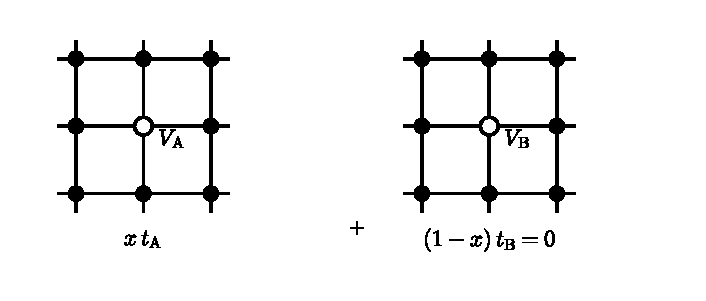
\includegraphics[width=8.5cm]{fig12-2.pdf}\\{\small 图 12.2\quad 二元无序合金中单格点近似的相干势近似的自洽方程图示（其中●组成待定的有效介质）}
\end{minipage}
\end{center}

再看无序系统的自能，在单格点近似时系统相对于有效介质的自能，可根据式(12.2.28)，写为
\begin{equation}
  \Sigma_{1}\left(\omega\right)=\frac{\langle t_{i}\rangle}
  {1+\mathscr{F}\left(\omega\right)\langle t_{i}\rangle}
\end{equation}
由 $\Sigma_{1}$ 构成的自能矩阵满足
\begin{equation}
  \hat{\boldsymbol{\Sigma}}_{1}=\hat{\boldsymbol{P}}^{-1}-\langle\hat{\boldsymbol{G}}\rangle^{-1}
\end{equation}
无序合金系统的自能矩阵则满足
\begin{equation}
  \hat{\boldsymbol{\Sigma}}=\hat{\boldsymbol{G}}_{0}^{-1}-\langle\hat{\boldsymbol{G}}\rangle^{-1}
\end{equation}
其中 $G_{0}$ 是 $H_{0}$ 的格林函数，不包括相干势 $u\left(\omega\right)$［见式(12.3.10)］.由于 $\hat{\boldsymbol{G}}_{0}^{-1}=\left(\omega\hat{\boldsymbol{I}}-\hat{\boldsymbol{H}}_{0}\right)$，而 $\hat{\boldsymbol{P}}^{-1}=\left(\omega\hat{\boldsymbol{I}}-\hat{\boldsymbol{H}}_{0}-u\hat{\boldsymbol{I}}\right)$.根据式(12.3.25)与式(12.3.26)，易求出 $\hat{\boldsymbol{\Sigma}}-\hat{\boldsymbol{\Sigma}}_{1}=u\left(\omega\right)\hat{\boldsymbol{I}}$.因此二元合金系统在单格点近似时的CPA自能为
\begin{equation}
  \Sigma\left(\omega\right)=u\left(\omega\right)+\Sigma_{1}\left(\omega\right)
\end{equation}
从 $\Sigma_{1}\left(\omega\right)$ 的表示式可知，当 $\langle t_{i}\left[u\left(\omega\right)\right]\rangle=0$ 时，$\Sigma_{1}\left(\omega\right)=0$.最后求得简单关系式
\begin{equation}
  \Sigma\left(\omega\right)=u\left(\omega\right)
\end{equation}
这是由于无序系统相对于有效介质的平均散射为零，因此有效介质的自能 $u\left(\omega\right)$ 就是无序系统的自能.相干势近似的成功就在于可以自洽决定相干势 $u\left(\omega\right)$，而 $u\left(\omega\right)$ 有自洽解则表明有效介质（或参考晶体）可以用一种规范的方法来自洽地确定，这就克服了平均t矩阵近似法不能自洽确定参考晶体的缺点.然而在相干势近似计算中，为了求得良好的近似解，从输入 $u\rightarrow$ 计算 $\mathscr{F}\left(\omega\right)\rightarrow$ 满足 $\langle t_{i}\rangle=0$ 条件往往需要多次反复进行，直至 $u\left(\omega\right)$ 满足相干势近似自洽方程式(12.3.21)为止.但是，这类自洽计算是可行的，因为在某些极限下系统有严格解.例如，在二元合金中当浓度 $x\rightarrow0$ 或 $x\rightarrow1$ 时，都可以找到严格解或良好近似解.

\subsection*{3. 简短结语}

相干势近似的中心思想是：将无规势用一个与频率 $\omega$ 有关，但具平移不变性的有效介质的相干势 $u\left(\omega\right)$ 来代替，后者由自洽条件决定.在单格点近似的CPA中，自洽条件要求无序系统与有效介质之间的散射t矩阵逐点平均为零，仅当此条件满足时才可求得如下重要结论：

（i）无规平均的格点格林函数等于有效介质的格林函数；

（ii）系统的自能就是有效介质的相干势.这时有效介质才是良好选择的.

无序系统中准粒子的态密度由无规平均格林函数的虚部决定
\begin{equation*}
  \rho\left(\omega\right)=-\left(1/\pi\right)\mathrm{Im}\left\{\left(1/N\right)\mathrm{Tr}\langle\hat{\boldsymbol{G}}\left(\omega+\mathrm{i}\eta\right)\rangle\right\}
\end{equation*}

{\sloppy
在相干势近似中，当 $\langle\hat{T}\rangle=0$ 时 $\langle\hat{\boldsymbol{G}}\rangle=\hat{\boldsymbol{P}}$，又因为 $\left(1/N\right)\mathrm{Tr}\left(\hat{\boldsymbol{P}}\right)=\mathscr{F}\left(\omega\right)$ $=\left(1/N\right)\sum_{k}\left[\omega-\varepsilon_{k}-u\left(\omega\right)\right]^{-1}$，这时准粒子的态密度简化为计算 $\mathscr{F}\left(\omega+\mathrm{i}\eta\right)$ 的虚部\par}
\begin{equation}
  \rho\left(\omega\right)=-\frac{1}{\pi}\mathrm{Im}\,\mathscr{F}\left(\omega+\mathrm{i}\eta\right)
\end{equation}
但应注意，在 $\mathscr{F}$ 中隐含相干势 $u\left(\omega\right)$，因此 $\mathscr{F}\left(\omega\right)$ 实际上代表 $\mathscr{F}\left[u\left(\omega\right)\right]$.相干势近似的自洽计算主要归结为求无序系统中准粒子的态密度 $\rho\left(\omega\right)$，并由此得知有关的热力学量.

相干势近似法不仅适用于在 $0<x<1$ 全浓度区求解成分（或替代）无序系统，它还因计入了多重散射效应可用于强散射体系.米泽曾对相干势近似方法作了详细的评述，有兴趣的读者可参阅文献[1].相干势近似已成为处理成分无序系统的一种行之有效的方法.在下节中，将介绍处理强关联电子系统的隶玻色子平均场近似法是如何被我们推广到无序系统的，并与相干势近似法相结合构成一个描述无序重费密子系统的强关联相干势近似理论\textsuperscript{[4,5]}.

\section{无序重费密子系统的相干势近似理论}

重费密子系统是每个元胞中均含局域f电子的晶格与传导电子的相互作用系统，其中同格点上f电子的强库仑排斥（即强关联）作用导致局域化，这是固体中首先涉及强关联电子体系的一个范例.正如上章中所指出重费密子系统包括金属与绝缘体两种情形，分别称为重费密子金属（如 $\mathrm{CeAl}_{3}$）和近藤绝缘体（如 $\mathrm{Ce}_{3}\mathrm{Bi}_{4}\mathrm{Pt}_{3}$），在理论上均可用安德逊晶格模型（ALM）描述.重费密子金属与近藤绝缘体的低温特性可运用处理强关联的隶玻色子平均场近似方法求解，并已在上章的§7与§8中作了详细的介绍.在本节中我们将讨论用La（无f电子）替代Ce（有f电子）所构成的无序重费密子系统，如重费密子合金 $\left(\mathrm{La}_{x}\mathrm{Ce}_{1-x}\right)\mathrm{Al}_{3}$ 和掺杂近藤绝缘体 $\left(\mathrm{La}_{x}\mathrm{Ce}_{1-x}\right)_{3}\mathrm{Bi}_{4}\mathrm{Pt}_{3}$ 等成分无序系统的CPA理论.

\subsection*{1. 重费密子系统的无序模型}

可将无序重费密子系统 $\left(\mathrm{La}_{x}\mathrm{Ce}_{1-x}\right)\mathrm{Al}_{3}$ 和 $\left(\mathrm{La}_{x}\mathrm{Ce}_{1-x}\right)_{3}\mathrm{Bi}_{4}\mathrm{Pt}_{3}$ 中的 $\left(\mathrm{La}_{x}\mathrm{Ce}_{1-x}\right)$ 部分看成二元无序合金 $\mathrm{A}_{x}\mathrm{B}_{1-x}$，其中A原子类La（不含f电子），B原子类Ce（含有f电子），其它部分仅提供传导电子并构成含f和c电子的无序系统.理论上相当于在安德逊晶格中的f部分引进成分无序.为此，定义i格点的无规变量
\begin{equation}
  \xi_{i}=\begin{cases}1 & \left(l\in\mathrm{A}\right)\\ 0 & \left(l\in\mathrm{B}\right)\end{cases}
\end{equation}
并注意到 $\xi_{i}$ 的无规平均 $\overline{\xi}_{i}^{2}=\overline{\xi}_{i}=x$，这里x代表合金中A原子的归一浓度.按此，可写出无序重费密子系统的出发哈密顿量
\begin{equation}
\begin{aligned}
  H&=\sum_{k,\sigma}\varepsilon_{k}C_{k\sigma}^{+}C_{k\sigma}
  +\sum_{i,\sigma}\left[\xi_{i}E_{\mathrm{L}}+\left(1-\xi_{i}\right)E_{0}\right]n_{i\sigma}^{f}
  +U\sum_{i}\left(1-\xi_{i}\right)n_{i\uparrow}^{f}n_{i\downarrow}^{f}\\
  &\quad+V\sum_{i,\sigma}\left(1-\xi_{i}\right)
  \left(C_{i\sigma}^{+}f_{i\sigma}+f_{i\sigma}^{+}C_{i\sigma}\right)
\end{aligned}
\end{equation}
其中 $n_{i\sigma}^{f}=f_{i\sigma}^{+}f_{i\sigma}$，$\varepsilon_{k}$ 为传导电子的能量，$E_{0}$ 是B原子上f电子的未微扰能级，它远在费密能级之下.$E_{\mathrm{L}}$ 代表A原子的f能级，为确保A上无f电子占据（类似La），在具体计算时应取 $E_{\mathrm{L}}\rightarrow\infty$.此外，V为安德逊c-f杂化参数，而U则是同一格点上自旋取向相反的f电子之间的库仑关联作用，这两项都只出现在被B原子（类Ce）占据的格点上.由于重费密子系统属于 $U\rightarrow\infty$ 强关联情形，这时B原子格点上f电子的双占据态将被严格排除，f电子的占据数只能取0或1，因此式中含U项将不出现.这时强关联效应可以通过在含V的杂化项中引入隶玻色子场算符 $b_{i}$ 并加上约束条件 $b_{i}^{+}b_{i}+\sum_{\sigma}f_{i\sigma}^{+}f_{i\sigma}=1$（其中 $i\in\mathrm{B}$）而严格计入.类似于上章§7中的讨论，作隶玻色子的平均场近似（SBMFA），引入隶玻色子的平均场参量 $\langle b_{i}\rangle=\langle b_{i}^{+}\rangle=r$ 和平均约束 $\lambda\sum_{i}\left(1-\xi_{i}\right)\left(r^{2}+\sum_{\sigma}f_{i\sigma}^{+}f_{i\sigma}-1\right)$，将SBMFA的无序哈密顿量写为
\begin{equation}
\begin{aligned}
  H_{\mathrm{MF}}&=\sum_{k\sigma}\varepsilon_{k}C_{k\sigma}^{+}C_{k\sigma}
  +\sum_{i\sigma}\left[\xi_{i}E_{\mathrm{L}}+\left(1-\xi_{i}\right)E_{0}\right]f_{i\sigma}^{+}f_{i\sigma}\\
  &\quad+rV\sum_{i\sigma}\left(1-\xi_{i}\right)
  \left(C_{i\sigma}^{+}f_{i\sigma}+f_{i\sigma}^{+}C_{i\sigma}\right)\\
  &\quad+\lambda\sum_{i}\left(1-\xi_{i}\right)
  \left(r^{2}+\sum_{\sigma}f_{i\sigma}^{+}f_{i\sigma}-1\right)
\end{aligned}
\end{equation}
注意在 $H_{\mathrm{MF}}$ 中无规变量 $\xi_{i}$ 既出现在f电子的格点能中，也出现在c-f杂化项中，这是一个既含“对角”又有“非对角”无序的系统.稍作整理可将 $H_{\mathrm{MF}}$ 中的无规部分写成下列（$2\times2$）矩阵表示：
\begin{equation}
\begin{aligned}
  H_{\mathrm{MF}}=\sum_{i,\sigma}\Bigl\{&\left(1-\xi_{i}\right)\left[C_{i\sigma}^{+}\ \ f_{i\sigma}^{+}\right]
  \begin{pmatrix}0 & rV\\ rV & E_{f}\end{pmatrix}
  \begin{pmatrix}C_{i\sigma}\\ f_{i\sigma}\end{pmatrix}\\
  &+\xi_{i}\left[C_{i\sigma}^{+}\ \ f_{i\sigma}^{+}\right]
  \begin{pmatrix}0 & 0\\ 0 & E_{\mathrm{L}}\end{pmatrix}
  \begin{pmatrix}C_{i\sigma}\\ f_{i\sigma}\end{pmatrix}\Bigr\}\\
  &+\sum_{k,\sigma}\varepsilon_{k}C_{k\sigma}^{+}C_{k\sigma}
  +\lambda\left(r^{2}-1\right)\left(1-x\right)N
\end{aligned}
\end{equation}
其中 $E_{f}=E_{0}+\lambda$ 代表f电子的重整能级，而SBMFA参量 $\lambda$ 与 $r$ 在i格点被B（类Ce）原子占据时满足与式(11.7.25)类似的自洽方程
\begin{equation}
  \left.
  \begin{aligned}
    r\lambda&=-V\sum_{\sigma}\ \langle C_{i\sigma}^{+}f_{i\sigma}\rangle\\
    1-r^{2}&=n_{f}=\sum_{\sigma}\ \langle f_{i\sigma}^{+}f_{i\sigma}\rangle
  \end{aligned}
  \right\}i\in\mathrm{B}
\end{equation}
在具体运算时，还需要作无规平均.

\subsection*{2. 有效介质}

由于 $H_{\mathrm{MF}}$ 中既含对角无序，又有非对角无序，并且可以用（$2\times2$）矩阵表示，应当引入下列（$2\times2$）的相干势作为有效介质的合理描述：
\begin{equation}
  S\left(\omega,x\right)=
  \begin{pmatrix}S_{\mathrm{cc}} & S_{\mathrm{cf}}\\ S_{\mathrm{fc}} & S_{\mathrm{ff}}\end{pmatrix}
\end{equation}
其中 $S\left(\omega,x\right)$ 与格点位置无关，这是一个具有平移对称性的待定函数，相干势矩阵的诸元素也与i无关，最多只是 $\omega$ 及x的函数.由此可写出有效介质的平均场哈密顿量
\begin{equation}
\begin{aligned}
  \overline{H}=\sum_{i,\sigma}\left[C_{i\sigma}^{+}\ \ f_{i\sigma}^{+}\right]
  &\begin{pmatrix}S_{\mathrm{cc}} & S_{\mathrm{cf}}\\ S_{\mathrm{fc}} & E_{f}+S_{\mathrm{ff}}\end{pmatrix}
  \begin{pmatrix}C_{i\sigma}\\ f_{i\sigma}\end{pmatrix}\\
  &+\sum_{k,\sigma}\varepsilon_{k}C_{k\sigma}^{+}C_{k\sigma}
  +\lambda\left(r^{2}-1\right)\left(1-x\right)N
\end{aligned}
\end{equation}
作傅里叶变换，可将这个待定的有效介质哈密顿量用布洛赫表象中算符表示
\begin{equation}
  \overline{H}=\sum_{k,\sigma}\left[C_{k\sigma}^{+}\ \ f_{k\sigma}^{+}\right]
  \begin{pmatrix}\varepsilon_{k}+S_{\mathrm{cc}} & S_{\mathrm{cf}}\\ S_{\mathrm{fc}} & E_{f}+S_{\mathrm{ff}}\end{pmatrix}
  \begin{pmatrix}C_{k\sigma}\\ f_{k\sigma}\end{pmatrix}
  +\lambda\left(r^{2}-1\right)\left(1-x\right)N
\end{equation}
将用于计算有效介质的平均格点格林函数.

现在讨论重费密子系统的相干势近似问题，首先由无序的 $H_{\mathrm{MF}}$ 与有效介质的 $\overline{H}$ 之差定义无规势
\begin{equation}
  H_{\mathrm{MF}}-\overline{H}\equiv\sum_{i}V_{i}
\end{equation}
对于二元无序合金，无规势只取两个分立值 $V_{\mathrm{A}}$ 和 $V_{\mathrm{B}}$，分别对应于取 $\xi_{i}$=1和0.根据式(12.4.4)和式(12.4.7)求得
\begin{equation}
  V_{\mathrm{A}}=
  \begin{pmatrix}-S_{\mathrm{cc}} & -S_{\mathrm{cf}}\\ -S_{\mathrm{fc}} & \varepsilon_{\mathrm{L}}-S_{\mathrm{ff}}\end{pmatrix},
  \qquad
  V_{\mathrm{B}}=
  \begin{pmatrix}-S_{\mathrm{cc}} & rV-S_{\mathrm{cf}}\\ rV-S_{\mathrm{fc}} & -S_{\mathrm{ff}}\end{pmatrix}
\end{equation}
在上式中 $\varepsilon_{\mathrm{L}}\equiv E_{\mathrm{L}}-E_{f}$，计算时可直接取 $\varepsilon_{\mathrm{L}}\rightarrow\infty$，它等效于 $E_{\mathrm{L}}\rightarrow\infty$.因为在上章§8中已证明：零温时，$E_{f}-\mu=k_{\mathrm{B}}T_{\mathrm{L}}$ 为小量，当取费密能（即零温化学势 $\mu$）为能量的原点时，有 $k_{\mathrm{B}}T_{\mathrm{L}}\ll E_{\mathrm{L}}$，这时 $\varepsilon_{\mathrm{L}}\rightarrow\infty$ 同样是保证A原子上无f电子的条件.根据式(12.2.26)，即可写出A、B原子在有效介质背景上的散射t矩阵
\begin{equation}
  t_{\mathrm{A}(\mathrm{B})}=V_{\mathrm{A}(\mathrm{B})}
  \left[1-F\left(\omega\right)V_{\mathrm{A}(\mathrm{B})}\right]^{-1}
\end{equation}
由此构成单格点近似的CPA自洽方程
\begin{equation}
  xt_{\mathrm{A}}+\left(1-x\right)t_{\mathrm{B}}=0
\end{equation}
其中 $F\left(\omega\right)$ 代表有效介质 $\overline{H}$ 的平均格点格林函数，可利用式(12.4.8)求出为
\begin{equation}
\begin{aligned}
  F\left(\omega\right)&=\frac{1}{N}\sum_{k}\overline{G}\left(\omega,\boldsymbol{k}\right)
  =\begin{pmatrix}F_{\mathrm{cc}} & F_{\mathrm{cf}}\\ F_{\mathrm{fc}} & F_{\mathrm{ff}}\end{pmatrix}\\
  &=\frac{1}{N}\sum_{k}
  \frac{\begin{pmatrix}\omega-E_{f}-S_{\mathrm{ff}} & S_{\mathrm{cf}}\\ S_{\mathrm{fc}} & \omega-\varepsilon_{k}-S_{\mathrm{cc}}\end{pmatrix}}
  {\left[\left(\omega-E_{f}-S_{\mathrm{ff}}\right)\left(\omega-\varepsilon_{k}-S_{\mathrm{cc}}\right)-S_{\mathrm{cf}}S_{\mathrm{fc}}\right]}
\end{aligned}
\end{equation}
当相干势 $S_{\mathrm{cc}}$、$S_{\mathrm{cf}}$、$S_{\mathrm{fc}}$ 和 $S_{\mathrm{ff}}$ 满足相干势近似自洽方程式(12.4.12)时，有效介质的格林函数 $\left[F\left(\omega\right)\right]$ 就是重费密子系统的无规平均格林函数.

\subsection*{3. 相干势的解}

联立式(12.4.10-13)，并取 $\varepsilon_{\mathrm{L}}\rightarrow\infty$ 条件后，经直接运算可证明在相干势矩阵 $S\left(\omega,x\right)$ 中有3个元素存在简单的解析解\textsuperscript{[4]}：
\begin{equation}
  S_{\mathrm{cc}}=0,\qquad S_{\mathrm{cf}}=S_{\mathrm{fc}}=rV
\end{equation}
只有 $S_{\mathrm{ff}}\left(\omega,x\right)$ 必须通过数值计算自洽求解.因此，相干势矩阵简化为
\begin{equation}
  S\left(\omega,x\right)=
  \begin{pmatrix}0 & rV\\ rV & S_{\mathrm{ff}}\left(\omega,x\right)\end{pmatrix}
\end{equation}
再将此解代入式(12.4.10)、(12.4.11)并取 $\varepsilon_{\mathrm{L}}\rightarrow\infty$，又可求出A、B原子相对有效介质的t矩阵解
\begin{equation}
  t_{\mathrm{A}}=\frac{1}{F_{\mathrm{ff}}\left(\omega\right)}
  \begin{pmatrix}0 & 0\\ 0 & -1\end{pmatrix},
  \qquad
  t_{\mathrm{B}}=\frac{S_{\mathrm{ff}}\left(\omega,x\right)}
  {1+S_{\mathrm{ff}}\left(\omega,x\right)F_{\mathrm{ff}}\left(\omega\right)}
  \begin{pmatrix}0 & 0\\ 0 & -1\end{pmatrix}
\end{equation}
最后，将 $t_{\mathrm{A}}$、$t_{\mathrm{B}}$ 解代入单格点近似的CPA自洽方程式(12.4.12)，求得简化的相干势近似自洽方程
\begin{equation}
  S_{\mathrm{ff}}\left(\omega,x\right)F_{\mathrm{ff}}\left(\omega\right)=-x
\end{equation}
其中与相干势 $S_{\mathrm{ff}}$ 同时自洽确定的 $F_{\mathrm{ff}}\left(\omega\right)$ 是f电子的平均格点格林函数
\begin{equation}
  F_{\mathrm{ff}}\left(\omega\right)=\frac{1}{N}\sum_{k}
  \frac{\left(\omega-\varepsilon_{k}\right)}
  {\left[\left(\omega-\varepsilon_{k}\right)\left(\omega-E_{f}-S_{\mathrm{ff}}\right)-\left(rV\right)^{2}\right]}
\end{equation}
由于我们找出了相干势的简单解式(12.4.15)，（$2\times2$）的相干势近似方程简化为仅仅求解一个未知相干势分量 $S_{\mathrm{ff}}$ 的问题，将使自洽计算的工作量明显减小.对应于相干势的简单解，$F\left(\omega\right)$ 矩阵的其它分量均可写成下列表示式：
\begin{equation}
  F_{\mathrm{cc}}\left(\omega\right)=\left(1/N\right)\sum_{k}
  \frac{\left(\omega-E_{f}-S_{\mathrm{ff}}\right)}
  {\left[\left(\omega-\varepsilon_{k}\right)\left(\omega-E_{f}-S_{\mathrm{ff}}\right)-\left(rV\right)^{2}\right]}
\end{equation}
\begin{equation}
  F_{\mathrm{fc}}\left(\omega\right)=F_{\mathrm{cf}}\left(\omega\right)
  =\frac{\left(rV\right)}{\left(\omega-E_{f}-S_{\mathrm{ff}}\right)}F_{\mathrm{cc}}\left(\omega\right)
\end{equation}
此外，无序重费密子系统的SBMFA参量 $\lambda$ 和 $r$ 所满足的方程式(12.4.5)经无规平均后，按照格林函数的谱定理，可用有效介质的平均格点格林函数表示为
\begin{equation}
  \left(1-x\right)r\lambda=\left(2/\pi\right)V\int_{-\infty}^{\infty}
  f\left(\omega-\mu\right)\mathrm{Im}\,F_{\mathrm{fc}}\left(\omega+\mathrm{i}\eta\right)\mathrm{d}\omega
\end{equation}
\begin{equation}
  \left(1-x\right)\left(1-r^{2}\right)=-\left(2/\pi\right)\int_{-\infty}^{\infty}
  f\left(\omega-\mu\right)\mathrm{Im}\,F_{\mathrm{ff}}\left(\omega+\mathrm{i}\eta\right)\mathrm{d}\omega
\end{equation}
其中 $f\left(\omega-\mu\right)$ 是费密分布函数，$\mu$ 为化学势，由总粒子数确定.设平均每格点的总电子浓度为 $n_{\mathrm{t}}=n_{\mathrm{c}}+n_{\mathrm{f}}$，其中 $n_{\mathrm{c}}$ 是传导电子的浓度，而f电子浓度在二元合金中为 $n_{\mathrm{f}}=\left(1-x\right)$.因此
\begin{equation}
\begin{aligned}
  n_{\mathrm{t}}=n_{\mathrm{c}}+\left(1-x\right)
  &=-\left(2/\pi\right)\int_{-\infty}^{\infty}\mathrm{d}\omega\,f\left(\omega-\mu\right)\\
  &\quad\times\mathrm{Im}\left[F_{\mathrm{cc}}\left(\omega+\mathrm{i}\eta\right)
  +F_{\mathrm{ff}}\left(\omega+\mathrm{i}\eta\right)\right]
\end{aligned}
\end{equation}
式(12.4.17)—(12.4.23)构成同时自洽决定无序重费密子系统的相干势 $S_{\mathrm{ff}}$，隶玻色子平均场参量r与 $\lambda$，以及化学势 $\mu$ 等未知量的基本方程组.此外，它还便于计算任意掺杂浓度x时的电子态密度.

\subsection*{4. 无序重费密子系统的电子态密度}

当自旋取向一定时，平均每个格点的传导电子态密度c-DOS由 $F_{\mathrm{cc}}\left(\omega+\mathrm{i}\eta\right)$ 的虚部直接决定
\begin{equation}
  \rho_{\mathrm{c}}\left(\omega,x\right)=-\left(1/\pi\right)\mathrm{Im}\,F_{\mathrm{cc}}\left(\omega+\mathrm{i}\eta\right)
  \qquad\left(\eta=0^{+}\right)
\end{equation}
而f-DOS表示平均每个B（类Ce）原子在确定自旋取向时的f电子态密度，它应由 $F_{\mathrm{ff}}\left(\omega+\mathrm{i}\eta\right)$ 的虚部决定
\begin{equation}
  \rho_{\mathrm{f}}\left(\omega,x\right)
  =-\left[1/\left(1-x\right)\pi\right]\mathrm{Im}\,F_{\mathrm{ff}}\left(\omega+\mathrm{i}\eta\right)
  \qquad\left(\eta=0^{+}\right)
\end{equation}
其中 $F_{\mathrm{ff}}$ 和 $F_{\mathrm{cc}}$ 由公式(12.4.18)，(12.4.19)决定.在计算时涉及将对k求和化为对能量的积分，还应给出传导电子的未微扰态密度
\begin{equation}
  \rho_{0}\left(\omega\right)=\left(1/N\right)\sum_{k}\delta\left(\omega-\varepsilon_{k}\right)
\end{equation}
{\sloppy
的具体形式.通常为方便起见，可取导带半宽为D的矩形态密度：$\rho_{0}\left(\omega\right)=\left(1/2D\right)$ $\left(|\omega|<D\right)$，$\rho_{0}\left(\omega\right)=0$ $\left(|\omega|>D\right)$.有时为表现细致特征，需采用更为合理的赫伯德型态密度：$\rho_{0}\left(\omega\right)=\left(2/\pi D\right)\left[1-\left(\omega/D\right)^{2}\right]^{1/2}$ $\left(|\omega|<D\right)$，$\rho_{0}\left(\omega\right)=0$ $\left(|\omega|>D\right)$.以上是无序重费密子系统中相干势近似理论的基本框架.\par}

在文献中常用未掺杂（即 $x=0$）时安德逊晶格中 $n_{\mathrm{c}}<1$ 或 $n_{\mathrm{c}}=1$ 而将有序的重费密子系统划分为重费密子金属和近藤绝缘体两大类：这种分类也被推广到无序体系，人们将 $n_{\mathrm{c}}<1$ 情形称为重费密子合金，而 $n_{\mathrm{c}}=1$ 情况则叫掺杂近藤绝缘体.对于掺杂近藤绝缘体系统，x代表掺入的类La原子（无f电子）浓度，由于用类La原子替代类Ce原子（有f电子）将产生缺少f电子的中心，形成近藤空穴，因此x又可称为近藤空穴的浓度.1994年我们应用上述相干势近似理论计算了掺杂近藤绝缘体系统中f-DOS随x的演化\textsuperscript{[4]}，结果表明：当未掺杂 $\left(x=0\right)$ 时，近藤绝缘体中在费密能级处存在如图11.15所示的非直接能隙，少量掺近藤空穴会在能隙的中央自然形成“隙间杂质带”，在中等掺杂时 $\left(x>10\%\mathrm{La}\right)$，能隙将被逐渐抹平，代之以双峰型的赝隙，表明系统已具有金属性.此结果可用于解释掺杂时随着x的增加，系统从近藤绝缘体向重费密子金属逐渐演变的实验现象.将此理论用于重费密子合金也对其低温相干特性作出了合理的说明\textsuperscript{[5]}.

在结束本节之前还需强调指出：无序重费密子系统不仅是强关联电子系统，而且还涉及强散射情形.这是因为用不含f电子的La取代含有f电子的Ce所形成的近藤空穴具有很高的能量 $\left(E_{\mathrm{L}}\rightarrow\infty\right)$，它远远高于Ce原子上f电子的能量 $\left(E_{\mathrm{L}}\gg|E_{0}|\right)$.因此，每个近藤空穴都是非常强的散射源，这时无序重费密子系统已不能用低阶玻恩近似作微扰处理，必须采用相干势近似，才能计入强散射源所导致的多重散射效应.这就是我们在SBMFA基础上构造相干势近似理论的初衷，在相关的文献中被称为推广的隶玻色子理论.

\section{无序系统中的电子态}

\subsection*{1. 安德逊的无序模型}

先定性介绍有序晶体与无序系统电子能态特征的主要区别.

具有严格周期性的有序晶格是平移不变的，单电子态可用波矢量 $\boldsymbol{k}$ 标记并形成能带，能带电子的状态由布洛赫函数表示
\begin{equation*}
  \psi_{\boldsymbol{k}}\left(\boldsymbol{r}\right)=u_{\boldsymbol{k}}\left(\boldsymbol{r}\right)\mathrm{e}^{\mathrm{i}\boldsymbol{k}\cdot\boldsymbol{r}}
\end{equation*}
所有的电子均在有序晶格中作公有化运动，且各格点周围振幅 $u_{\boldsymbol{k}}\left(\boldsymbol{r}\right)$ 相同，这种状态在整个晶体中的扩展特征是长程序效应的反映，因此布洛赫态又可称为扩展态（extended states）.具有扩展态是有序晶格的特点.

当有序晶格中（如半导体）掺入少量杂质后，周期性被局部破坏，正如第八章中讨论所指出，这时将有电子或空穴被束缚在杂质上，并在导带之下或价带之上（能隙区中）形成施主和受主能级，这些电子（或空穴）的波函数是指数衰减型的定域函数
\begin{equation*}
  \psi\left(\boldsymbol{r}\right)\sim\exp\left(-r/\zeta\right)
\end{equation*}
$\zeta$ 称为定域化长度.这时电子在杂质附近作定域化的运动，有别于扩展在整个晶体中的公有化运动，称为电子的定域态（localized states，又称局域态）.实验表明当杂质浓度增高时，定域态的电子能级可能密集成带，并与导带相连接，形成导带的尾部（tail），它们对电导率的贡献很小\textsuperscript{[6]}.由此可知存在定域态是无序的标志.

对于无序系统的电子态理论研究有两种处理方法：其一是对无序系统作某种平均后近似当作有序系统来处理，这种方法以相干势近似为代表.其二，则相反的从无序系统的定域态特点出发，设计一些无序模型，研究无序系统与有序系统电子态的差别，这种方法以安德逊的工作为代表，最简单的介绍可参考李雅达的报告\textsuperscript{[7]}.我们将用比文献[7]稍为严格一些的方法介绍安德逊工作，首先引进安德逊的无序模型.

与有序晶格不同，无序系统由于不具有平移对称性，波矢量 $\boldsymbol{k}$ 不再是描述电子状态的好量子数，我们必须从定域态（或原子轨道态）出发设计模型和讨论问题.安德逊将紧束缚近似（TBA）方法推广用于无序系统，设单电子哈密顿量为
\begin{equation}
  H=-\frac{\hbar^{2}}{2m}\nabla^{2}+V\left(\boldsymbol{r}\right)
\end{equation}
取瓦尼尔函数 $a\left(\boldsymbol{r}-\boldsymbol{l}\right)$ 为基，将二次量子化态向量表示成
\begin{equation*}
  \Psi\left(\boldsymbol{r}\right)=\sum_{l}C_{l}\,a\left(\boldsymbol{r}-\boldsymbol{l}\right)
\end{equation*}
则H可改写为
\begin{equation}
  H=\sum_{l}\mathscr{E}_{l}C_{l}^{+}C_{l}+\sum_{l\neq l'}\ \sum_{l'}V_{ll'}C_{l}^{+}C_{l'}
\end{equation}
其中
\begin{equation}
  \mathscr{E}_{l}\equiv H_{ll}=\int a^{*}\left(\boldsymbol{r}-\boldsymbol{l}\right)
  Ha\left(\boldsymbol{r}-\boldsymbol{l}\right)\mathrm{d}\tau
\end{equation}
代表l格点附近定域电子能量，而 $V_{ll'}$ 就是交迭积分
\begin{equation}
  V_{ll'}\equiv H_{ll'}=\int a^{*}\left(\boldsymbol{r}-\boldsymbol{l}\right)
  Ha\left(\boldsymbol{r}-\boldsymbol{l}'\right)\mathrm{d}\tau
\end{equation}
在TBA范围内 $V_{ll'}=V_{l}\delta_{l',l+h}$，$\boldsymbol{h}$ 为近邻格点间位置矢差，$V_{l}$ 代表l格点处电子的近邻交迭积分.

当系统为有序晶格时，由于具有平移对称性可引入波矢 $\boldsymbol{k}$ 描述电子状态，并利用布洛赫定理得到 $C_{k}$ 与 $C_{l}$ 的关系为
\begin{equation}
  C_{l}=\frac{1}{\sqrt{N}}\sum_{k}\mathrm{e}^{\mathrm{i}\boldsymbol{k}\cdot\boldsymbol{l}}C_{k}
\end{equation}
这个关系只适用于有序或近似有序的晶格.另外，由于平移对称各格点的 $\mathscr{E}_{l}$ 及 $V_{l}$ 均与l无关，可令 $\mathscr{E}_{l}=\mathscr{E}_{0}$ 以及 $V_{l}=V$，式(12.5.4)简化为
\begin{equation}
  V_{ll'}=V\delta_{l',l+h}
\end{equation}
V代表近邻交迭积分.系统的哈密顿量简化为 $C_{k}$ 的对角形式
\begin{equation}
\begin{aligned}
  H&=\mathscr{E}_{0}\sum_{l}C_{l}^{+}C_{l}
  +V\sum_{l}\ \sum_{h}C_{l}^{+}C_{l+h}\\
  &=\sum_{k}E\left(\boldsymbol{k}\right)C_{k}^{+}C_{k}
\end{aligned}
\end{equation}
其中
\begin{equation}
  E\left(\boldsymbol{k}\right)=\mathscr{E}_{0}+V\sum_{h}\mathrm{e}^{\mathrm{i}\boldsymbol{k}\cdot\boldsymbol{h}}
\end{equation}
这就是TBA的能带电子能量，其能带宽度等于 $2Z|V|$，Z是配位数.若取带中心能量 $\mathscr{E}_{0}$ 为原点，则有序晶格的电子态能量
\begin{equation}
  E\left(\boldsymbol{k}\right)=V\sum_{h}\mathrm{e}^{\mathrm{i}\boldsymbol{k}\cdot\boldsymbol{h}}
\end{equation}
相当于令 $\mathscr{E}_{0}=0$.

对于无序系统，$\mathscr{E}_{l}$ 将随格点l作随机变化，这时不能再令 $\mathscr{E}_{l}=0$，安德逊假定 $\mathscr{E}_{l}$ 在W宽度内是连续均匀分布的，各格点上的 $\mathscr{E}_{l}$ 是独立无规变量，其分布概率为
\begin{equation}
  P\left(\mathscr{E}_{l}\right)=
  \begin{cases}
    \dfrac{1}{W} & \left(|\mathscr{E}_{l}|\leqslant\dfrac{W}{2}\right)\\[0.8em]
    0 & \left(|\mathscr{E}_{l}|>\dfrac{W}{2}\right)
  \end{cases}
\end{equation}
如图12.3所示.对于近邻交迭积分，假设它仍与l无关由V表示，式(12.5.6)仍然适用，这就是安德逊设计的无序模型.在安德逊模型中哈密顿量写成
\begin{equation}
  H=\sum_{l}\mathscr{E}_{l}C_{l}^{+}C_{l}
  +V\sum_{l}\ \sum_{h}C_{l}^{+}C_{l+h}
\end{equation}

\begin{center}
\begin{minipage}{6cm}
\centering
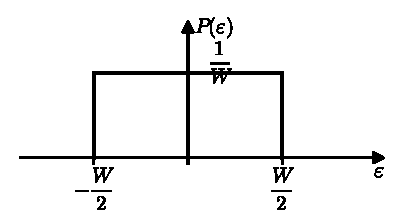
\includegraphics[width=6cm]{fig12-3.pdf}\\{\small 图 12.3}
\end{minipage}
\end{center}

其中无规变量是 $\mathscr{E}_{l}$，它的变化宽度W可当作反映系统“无序程度”的参量，而各格点的近邻交迭积分均取相同值V则表示无序系统的“短程有序”特性.因此，这个简化的模型概括了无序系统的主要特点.由此出发将便于求得定域化条件和引进迁移率边界等新概念.

\subsection*{2. 安德逊定域化\textsuperscript{[8]}}

安德逊首先对无序系统中的电子定域态和扩展态作了严格定义.他指出，在无限大的体系中\footnote{由于无序系统不存在平移对称性，人们不必像有序晶体那样去设计周期性边界条件，以保证有限晶体的平移对称性，而是直接讨论无限大样品的热力学极限（$N\rightarrow\infty$，$V\rightarrow\infty$ 和 $N/V=$ 有限）.}设 $t=0$ 时l格上（或其附近）有一个电子，那么经过较长时间t以后在l格点上如果找到这个电子的概率振幅 $A_{l}\left(t\right)$ 为零，就说明电子离开了这个格点在系统中传播，电子处于扩展态；如果 $A_{l}\left(t\right)\neq0$（t很大），就表示电子在l格点附近形成了稳定的定域态，这就是安德逊的定域化概念.

安德逊详细讨论了这个含时问题，得到的结论是：对于三维无序系统，当无规起伏势能的分布宽度W与带宽2ZV之比 $\delta$ 大于某个临界值 $\delta_{\mathrm{c}}$ 时，无序系统中所有的本征态都是定域态，$\delta_{\mathrm{c}}$ 的数值大致等于2.

利用 $C_{l}$ 及 $C_{l'}^{+}$ 所组成的双时推迟格林函数
\begin{equation}
  G_{ll'}\left(t\right)\equiv-\mathrm{i}\theta\left(t\right)
  \langle\left[C_{l}\left(t\right),\,C_{l'}^{+}\left(0\right)\right]_{+}\rangle
\end{equation}
讨论安德逊模型是方便的.当 $T=0$ K时上式简化为对基态的平均
\begin{equation}
  G_{ll'}\left(t\right)=-\mathrm{i}\theta\left(t\right)
  \langle0|C_{l}\left(t\right)C_{l'}^{+}\left(0\right)|0\rangle
\end{equation}
这个函数的对角部分 $G_{ll}\left(t\right)$ 直接与 $A_{l}\left(t\right)$ 有关，因为 $\mathrm{i}G_{ll}\left(t\right)$ 正好就是 $t=0$ 时刻在l格点上产生一个电子，经t时间后 $\left(t>0\right)$ 在同一格点上找到这个电子的概率振幅 $A_{l}\left(t\right)$
\begin{equation}
  A_{l}\left(t\right)=\langle0|C_{l}\left(t\right)C_{l}^{+}\left(0\right)|0\rangle
  =\mathrm{i}G_{ll}\left(t\right)\qquad\left(t>0\right)
\end{equation}
因此，只要解出对角格林函数 $G_{ll}\left(t\right)$，就可以讨论定域化条件.

具体的做法是：利用TBA哈密顿量式(12.5.2)和
\begin{equation}
  \mathrm{i}\dot{C}_{l}=\left[C_{l},H\right],\qquad
  \left[C_{l},C_{l'}^{+}\right]_{+}=\delta_{ll'}
\end{equation}
写出 $G_{ll'}\left(t\right)$ 的运动方程
\begin{equation}
  \mathrm{i}\dot{G}_{ll'}\left(t\right)=\delta\left(t\right)\delta_{ll'}
  +\mathscr{E}_{l}G_{ll'}\left(t\right)
  +\sum_{l''\left(l''\neq l\right)}V_{ll''}G_{l''l'}\left(t\right)
\end{equation}
其中 $\delta\left(t\right)$ 来源于 $\theta\left(t\right)$ 对时间求导.再作傅里叶变换
\begin{equation}
  G_{ll'}\left(t\right)=\frac{1}{2\pi}\int_{-\infty}^{\infty}
  \mathrm{d}E\,\mathrm{e}^{-\mathrm{i}Et}G_{ll'}\left(E\right)
\end{equation}
和
\begin{equation}
  \delta\left(t\right)=\frac{1}{2\pi}\int_{-\infty}^{\infty}\mathrm{d}E\,\mathrm{e}^{-\mathrm{i}Et}
\end{equation}
将运动方程式(12.5.16)用 $G_{ll'}\left(E\right)$ 格林函数表示为更简单形式
\begin{equation}
  \left(E-\mathscr{E}_{l}\right)G_{ll'}\left(E\right)=\delta_{ll'}
  +\sum_{l''\left(l''\neq l\right)}V_{ll''}G_{l''l'}\left(E\right)
\end{equation}
定义
\begin{equation}
  g_{l}\equiv\frac{1}{E-\mathscr{E}_{l}}
\end{equation}
它代表自由格林函数，立刻求得全格林函数 $G_{ll'}\left(E\right)$ 满足下列积分方程式：
\begin{equation}
  G_{ll'}\left(E\right)=g_{l}\delta_{ll'}
  +\sum_{l''\left(l''\neq l\right)}g_{l}V_{ll''}G_{l''l'}\left(E\right)
\end{equation}
由于 $G_{ll'}\left(E\right)$ 是推迟格林函数，其中E代表 $E+\mathrm{i}\eta$，$\eta=+0$.

全对角格林函数 $G_{ll}\left(E\right)$ 的运动方程可写成
\begin{equation}
  \left(E-\mathscr{E}_{l}\right)G_{ll}\left(E\right)=1
  +\sum_{l'\left(l'\neq l\right)}V_{ll'}G_{l'l}\left(E\right)
\end{equation}
将式(12.5.21)代入式(12.5.22)，经整理后得
\begin{equation}
\begin{aligned}
  &\left\{E-\mathscr{E}_{l}-\sum_{l'\left(l'\neq l\right)}V_{ll'}g_{l'}V_{l'l}\right\}G_{ll}\left(E\right)\\
  &\qquad=1+\sum_{l'\left(l'\neq l\right)}\ \sum_{l''\left(l''\neq l,l'\right)}
  V_{ll'}g_{l'}V_{l'l''}g_{l''}G_{l''l}\left(E\right)
\end{aligned}
\end{equation}
再利用式(12.5.21)作逐次迭代，最后可求得对角格林函数满足方程
\begin{equation}
  \left\{E-\Sigma\left(l;E\right)\right\}G_{ll}\left(E\right)=1
\end{equation}
其中
\begin{equation}
\begin{aligned}
  \Sigma\left(l;E\right)&=\mathscr{E}_{l}
  +\sum_{l'\left(l'\neq l\right)}V_{ll'}g_{l'}V_{l'l}\\
  &\quad+\sum_{l'\left(l'\neq l\right)}\ \sum_{l''\left(l''\neq l,l'\right)}
  V_{ll'}g_{l'}V_{l'l''}g_{l''}V_{l''l}+\cdots
\end{aligned}
\end{equation}
$\Sigma\left(l;E\right)$ 称为自能，它代表全对角格林函数
\begin{equation}
  G_{ll}\left(E\right)=\frac{1}{\left\{E-\Sigma\left(l;E\right)\right\}}
\end{equation}
的极点，根据 $G_{ll}\left(E\right)$ 在复平面上的解析性质可以决定 $A_{l}\left(t\right)$.如果自能 $\Sigma\left(l;E\right)$ 的微扰展开级数式(12.5.25)在实轴上收敛，并设其取值为 $E_{0}$，则 $G_{ll}\left(E+\mathrm{i}\eta\right)$ 的极点在 $E_{0}+\mathrm{i}\eta$，它随 $\eta\rightarrow+0$ 趋向实轴，根据式(12.5.14)和(12.5.17)
\begin{equation}
  A_{l}\left(t\right)=\mathrm{i}G_{ll}\left(t\right)=\frac{\mathrm{i}}{2\pi}\int_{-\infty}^{\infty}
  \mathrm{d}E\,\frac{\mathrm{e}^{-\mathrm{i}Et}}{E-E_{0}+\mathrm{i}\eta}
  \sim\mathrm{e}^{-\mathrm{i}E_{0}t}
\end{equation}
当 $t\rightarrow\infty$，$A_{l}\left(t\right)\neq0$，按照前面的讨论，这里在l格点附近形成了稳定的局域态.因此，$\Sigma\left(l;E\right)$ 微扰级的收敛条件就是E能量上形成电子定域态的判据.

利用式(12.5.6)，将相干势近似的自能写成
\begin{equation}
\begin{aligned}
  \Sigma\left(l;E\right)&=\mathscr{E}_{l}
  +\sum_{r}Vg_{r}V+\sum_{r}\ \sum_{r}Vg_{r}Vg_{r}V+\cdots\\
  &=\mathscr{E}_{l}+V\sum_{L=1}^{\infty}\ \sum_{j}T_{j}^{(L)}
\end{aligned}
\end{equation}
其中级数的一般项
\begin{equation}
  T_{j}^{(L)}\equiv\frac{V^{L}}{\left(E-\mathscr{E}_{l_{1}}\right)\cdots\left(E-\mathscr{E}_{l_{L}}\right)}
  =\prod_{i=1}^{L}\ Vg_{l_{i}}
\end{equation}
代表从l格点出发经过 $l_{1},\cdots,l_{L}$ 个不同格点再回到l，其中 $l_{1},\cdots,l_{L}$ 不能重复\footnote{这种只有最后才回到l的求和途径称为自回避路径（self-avoiding walk）.}.由于每个格点有Z个近邻，与 $T_{j}^{(L)}$ 相似的L阶项大致有 $Z^{L}$ 个，包括在求和j中.又由于 $g_{l_{i}}=\left(E-\mathscr{E}_{l_{i}}\right)^{-1}$ 中 $\mathscr{E}_{l_{i}}$ 是无规分布的，式(12.5.29)是一个随机级数，其收敛条件必须通过概率的统计决定\textsuperscript{[9]}.在这里我们将介绍席曼（Ziman）\textsuperscript{[10]}的简单估计，其优点是可以同时导出迁移率边界.

席曼讨论 $\bigl|T_{j}^{(L)}\bigr|$ 的对数函数，定义
\begin{equation}
  Q\equiv\ln\bigl|T_{j}^{(L)}\bigr|
  =\ln\prod_{i=1}^{L}\ \bigl|Vg_{l_{i}}\bigr|
  =\sum_{i=1}^{L}\ln\ \bigl|Vg_{l_{i}}\bigr|
\end{equation}
由于 $T_{j}^{(L)}$ 中 $l_{i}$ 取不同格点，$g_{l_{i}}$ 无规变化，$\ln|Vg_{l_{i}}|$ 可用无规平均 $\langle\ln|Vg_{l_{i}}|\rangle$ 代表
\begin{equation}
  \langle\ln|Vg_{l_{i}}|\rangle=\int\mathrm{d}\mathscr{E}_{l_{i}}\,
  P\left(\mathscr{E}_{l_{i}}\right)\ln\left|\frac{V}{E-\mathscr{E}_{l_{i}}}\right|
\end{equation}
$P\left(\mathscr{E}\right)$ 是安德逊模型所取的分布，式(12.5.10).显然，$\langle\ln|Vg_{l_{i}}|\rangle$ 与格点无关，可简记为 $\langle\ln|Vg|\rangle$.因此，就统计平均讲
\begin{equation}
  Q\approx\sum_{i=1}^{L}\ln\bigl|Vg_{l_{i}}\bigr|
  \approx L\langle\ln|Vg|\rangle
\end{equation}
而
\begin{equation}
  \bigl|T_{j}^{(L)}\bigr|=\mathrm{e}^{Q}
  =\exp\Bigl\{\sum_{i=1}^{L}\ln\bigl|Vg_{l_{i}}\bigr|\Bigr\}
  \approx\exp\left\{L\langle\ln|Vg|\rangle\right\}
\end{equation}
由于有 $Z^{L}$ 项与 $\bigl|T_{j}^{(L)}\bigr|$ 形式相同，根据上式求得
\begin{equation}
  \sum_{j}\ \bigl|T_{j}^{(L)}\bigr|
  \approx\left\{Z\exp\left(\langle\ln|Vg|\rangle\right)\right\}^{L}
\end{equation}
考虑到自能函数 $\Sigma\left(l;E\right)$ 的级数一般项 $T_{j}^{(L)}$ 可正可负，应有
\begin{equation}
  \sum_{j}T_{j}^{(L)}<\sum_{j}\ \bigl|T_{j}^{(L)}\bigr|
\end{equation}
因此席曼指出，自能级数 $\Sigma\left(l;E\right)$ 的收敛性不会比下列几何级数的收敛性差
\begin{equation}
  \mathscr{E}_{l}+V\sum_{L=1}^{\infty}
  \left\{Z\exp\left(\langle\ln|Vg|\rangle\right)\right\}^{L}
\end{equation}
我们可以用这个级数的收敛条件
\begin{equation}
  Z\exp\left(\langle\ln|Vg|\rangle\right)<1
\end{equation}
作为 $\Sigma\left(l;E\right)$ 级数的绝对收敛条件，即形成定域态的条件.将 $P\left(\mathscr{E}\right)$ 分布和式(12.5.10)代入无规平均公式(12.5.31)中，容易算出
\begin{equation}
\begin{aligned}
  \phi\left(E\right)&\equiv\langle\ln|Vg|\rangle
  =\frac{1}{W}\int_{-W/2}^{W/2}\ln\left|\frac{V}{E-\mathscr{E}}\right|\mathrm{d}\mathscr{E}\\
  &=1-\frac{1}{2}\Bigl\{\left(1+\frac{2E}{W}\right)\ln\left|\frac{W}{2V}+\frac{E}{V}\right|
  +\left(1-\frac{2E}{W}\right)\ln\left|\frac{W}{2V}-\frac{E}{V}\right|\Bigr\}
\end{aligned}
\end{equation}
对于 $E=0$ 态
\begin{equation*}
  \phi\left(0\right)=1-\ln\left|\frac{W}{2V}\right|
\end{equation*}
代入收敛条件式(12.5.37)，即可求得 $E=0$ 态的定域化条件为
\begin{equation}
  \delta\equiv\frac{W}{2Z|V|}>\mathrm{e}
\end{equation}
其临界值 $\delta_{\mathrm{c}}=\mathrm{e}=2.7\cdots$，与安德逊结果一致\textsuperscript{[8]}.由于 $E=0$ 时，$\langle\ln|Vg|\rangle$ 取值最大，当 $E=0$ 态成为定域态时，三维无序系统的其它本征态 $\left(|E|>0\right)$ 必然都能满足收敛条件 $Z\exp\left(\langle\ln|Vg|\rangle\right)<1$，因此当 $\delta>\delta_{\mathrm{c}}$ 时无序系统中所有的本征态都是定域态，这就是安德逊的结论，式(12.5.39)常称为安德逊定域化条件.

应当指出，在安德逊模型中 $P\left(\mathscr{E}\right)$ 取矩形分布纯粹是为了数学处理方便，它并不影响安德逊结论的普遍性.如果采用半带宽为 $\Gamma$ 的洛仑兹型分布
\begin{equation}
  P\left(\mathscr{E}\right)=\frac{ZV}{\left(\mathscr{E}^{2}+\Gamma^{2}\right)^{1/2}}
\end{equation}
同样也可证明安德逊定域化条件\textsuperscript{[11]}.

\subsection*{3. 莫特模型}

当 $\delta<\delta_{\mathrm{c}}$ 时，三维无序系统中 $E=0$ 态不满足收敛条件，它不能形成稳定的定域态，仍是在系统中传播的扩展态.莫特\textsuperscript{[6]}指出：这时在无序系统中既存在扩展态，也存在定域态.扩展态分布于紧束缚近似能带中心，定域态在带尾部分，并有一个划分扩展态与定域态的能量分界 $E_{\mathrm{c}}$，如图12.4所示.当 $|E|<|E_{\mathrm{c}}|$ 时为扩展态，$|E|>|E_{\mathrm{c}}|$ 时为定域态.当温度趋向于0 K时定域态中电子迁移率趋向零，而扩展态中迁移率仍为有限值，因此莫特将 $E_{\mathrm{c}}$ 称为迁移率边缘.

\begin{center}
\begin{minipage}{7cm}
\centering
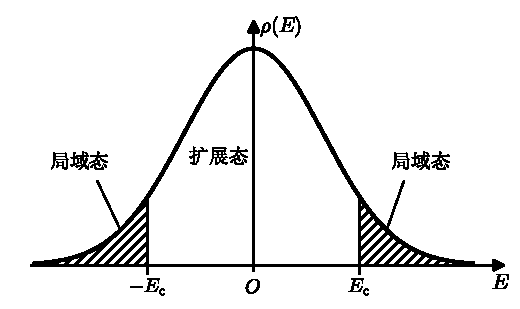
\includegraphics[width=7cm]{fig12-4.pdf}\\{\small 图 12.4\quad $\delta<\delta_{\mathrm{c}}$ 时的电子态密度}
\end{minipage}
\end{center}

利用席曼结果式(12.5.38)，很容易证实莫特的上述设想.因为 $\phi\left(E\right)\equiv\langle\ln|Vg|\rangle$ 与E的关系已求出，将它代入自能 $\Sigma\left(l;E\right)$ 的收敛条件式(12.5.37)，就可以求得任意E态的定域化条件为
\begin{equation}
  \delta=\frac{W}{2Z|V|}>\delta_{\mathrm{c}}\left(E\right)
  \equiv\frac{e}{\left|1-\left(\frac{2E}{W}\right)^{2}\right|^{1/2}}
  \left|\frac{1-\frac{2E}{W}}{1+\frac{2E}{W}}\right|^{\frac{E}{W}}
\end{equation}
对于给定 $\delta$（即W与 $|V|$）的无序系统，当 $\delta$ 略小于 $\mathrm{e}\equiv\delta_{\mathrm{c}}\left(0\right)$ 时，在紧束缚近似能带范围 $\left(|E|\leqslant Z|V|\right)$ 内的状态限于 $\dfrac{2|E|}{W}<\dfrac{1}{\mathrm{e}}$，这时 $\delta_{\mathrm{c}}\left(E\right)$ 将随 $|E|$ 增大而减少，因此 $|E|$ 超过某能量界 $|E_{\mathrm{c}}|$ 的电子态能够满足定域化条件式(12.5.41)，说明无序将使紧束缚近似能带的部分扩展态变为定域态，局域态靠近带边，扩展态在带中心附近.此外，对于无序系统当然还应存在 $|E|>Z|V|$ 的本征态，它与带边相接形成带尾，带尾中状态也是定域态.莫特在此基础上指出，对于非晶态半导体，由于势场的无规起伏还没有达到临界值 $\delta_{\mathrm{c}}\left(0\right)$，因而在非晶半导体中同时存在电子的定域态和扩展态，也存在它们之间的明显分界 $E_{\mathrm{c}}$——迁移率边界，这就是非晶态半导体的莫特模型.

莫特还进一步提出了安德逊转变（Anderson transition）\textsuperscript{[12]}的概念，如果在Si晶体中掺入施主杂质磷（P，5价），由于施主杂质的分布是无规的，就形成无序系统，无序性将导致有一个迁移率边缘，设导带中电子的费密能 $E_{\mathrm{F}}$ 位于迁移率边缘之下（从导带底看），此时系统中电子态都是定域态，可认为是一个“绝缘体”.如果继续掺杂，使费密能级通过迁移率边缘，位于它的上面，系统将表现出“金属性”，因为在扩展态上占有电子.这里发生了从绝缘体向金属的转变，称为安德逊转变.安德逊转变来源于无序效应，它与第十一章§1中所介绍的莫特转变不同，莫特转变是电子间关联作用导致的金属-绝缘体转变.

应当指出，莫特模型仍然存在着争议，争论的焦点在于是否存在迁移率边界.根据莫特的观点，随着无序度 $\delta$ 增大，系统的电导率将减小，在临界值 $\delta_{\mathrm{c}}$ 处电导率有一个跳跃，从有限值变为零，在这里存在着扩展态的最小电导率 $\sigma_{\mathrm{min}}$.目前，关于是否有 $\sigma_{\mathrm{min}}$ 的问题在实验和理论上都还存在分歧，是一个尚未争论清楚的问题\textsuperscript{[13]}.

近年来，人们把无序系统的定域态与扩展态类比的看成为两相，借助于处理相变和临界现象的强有力工具，发展了安德逊定域化的标度理论\textsuperscript{[14]}.标度理论证明了：在一维无序系统中，任何小的无序都会导致局域化.在二维情况下理论也肯定了定域态，至于是否存在扩展态尚有争议.至于三维情况，一般都认为有定域态，有扩展态，也有临界的 $\delta_{\mathrm{c}}$ 值.标度理论所求得的 $\delta_{\mathrm{c}}$ 值大致为1，比安德逊和席曼的估计值小2至3倍，看来是比较合理的结果\textsuperscript{[15]}.关于定域化的标度理论将在本章§8中介绍.

\section{定程与变程跳跃电导}

根据上节的讨论，当费密能级 $E_{\mathrm{F}}$ 位于迁移率边界 $E_{\mathrm{c}}$ 之下 $\left(E_{\mathrm{F}}<E_{\mathrm{c}}\right)$ 时，系统中所有的电子均处于定域态，这些定域态的能量无规地分布在相当宽的能量范围内，相邻的定域中心之间往往有较大的能量差，只有在更远的距离才可能找到能量相近的定域中心，如图12.5所示.对于这样一个全由定域态组成的系统，其零温电导率 $\sigma=0$，属于绝缘体.在有限温度T时，电子才可以通过热激活吸收声子的能量，从一个定域中心隧穿到另一个定域中心，产生跳跃电导.换句话说，跳跃（hopping）是指电子从一个定域态到另一个定域态借助声子进行的量子力学隧穿过程\textsuperscript{[16]}.跳跃电导包括两种传导过程：其一是电子的跃迁主要发生在最近邻的定域中心之间，称为定程跳跃电导.其二是电子的转移发生在相距更远、能量差别较小的两个定域中心之间.莫特（Mott）\textsuperscript{[17]}首先研究了这种新的跳跃传导过程，并求出了其最可几的跳迁距离是随温度T变化的，被称为莫特变程跳跃电导.

\begin{center}
\begin{minipage}{7.5cm}
\centering
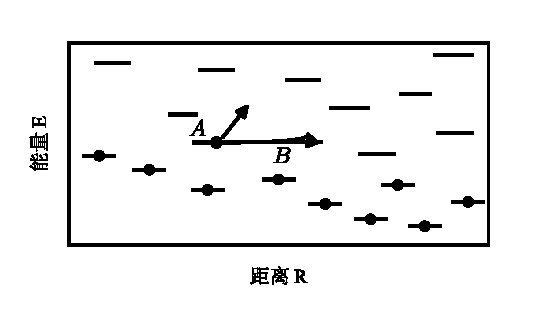
\includegraphics[width=7.5cm]{fig12-5.pdf}\\{\small 图 12.5\quad 定域态间的跳跃传导示意图}
\end{minipage}
\end{center}

现在讨论位于 $\boldsymbol{R}_{i}$ 和 $\boldsymbol{R}_{j}$，能量分别为 $E_{i}$ 和 $E_{j}\ \left(E_{j}>E_{i}\right)$ 的两个定域态之间的电子跃迁.根据量子力学，电子从 $\boldsymbol{R}_{i}$ 中心，经过距离 $R=|\boldsymbol{R}_{i}-\boldsymbol{R}_{j}|$ 隧穿到 $\boldsymbol{R}_{j}$ 中心的概率正比于i与j定域态间波函数的交迭积分之平方.对于定域态，$\phi\left(\boldsymbol{r}-\boldsymbol{R}_{i}\right)\propto\exp\left(-|\boldsymbol{r}-\boldsymbol{R}_{i}|/\lambda\right)$，其中 $\lambda$ 为局域化长度.当两定域态的局域化长度近似相同时，交换积分可表示为
\begin{equation}
  \int\psi^{*}\left(\boldsymbol{r}-\boldsymbol{R}_{i}\right)\psi\left(\boldsymbol{r}-\boldsymbol{R}_{j}\right)\mathrm{d}^{3}r
  \propto\exp\left(-R/\lambda\right)
\end{equation}
因此，$\boldsymbol{R}_{i}$ 与 $\boldsymbol{R}_{j}$ 定域态间的隧穿概率正比于 $\exp\left(-2\alpha R\right)$，其中 $\alpha^{-1}\equiv\lambda$.另一方面，由于两定域态的能量不相同，从 $\boldsymbol{R}_{i}$ 跃迁到 $\boldsymbol{R}_{j}$ 所需的能 $W=E_{j}-E_{i}\ \left(>0\right)$ 必须由热声子供给.因此，在 $T=0$ K时，尽管相邻的定域态之间波函数有明显的重叠，但由于没有热声子的供给，电子无法克服两个定域态之间的能量差W，其实际的跃迁概率仍为零.这就是当 $T=0$ K时定域态系统的电子导率为零的物理原因.仅当温度为有限时，由于具有W能量的热声子数为 $\left[\exp\left(W/k_{\mathrm{B}}T\right)-1\right]^{-1}$，它在 $k_{\mathrm{B}}T\ll W$ 时可用玻耳兹曼因子 $\exp\left(-W/k_{\mathrm{B}}T\right)$ 表示，这时借助于声子供给能量才可能发生跳跃电导.因此，从 $\boldsymbol{R}_{i}$ 到 $\boldsymbol{R}_{j}$ 的跳跃概率不仅正比于隧穿概率 $\exp\left(-2\alpha R\right)$，还应当正比于辅助这一跳跃传导的热平衡声子数 $\exp\left(-W/k_{\mathrm{B}}T\right)$，并写成
\begin{equation}
  w_{ij}=w_{0}\exp\left(-2\alpha R-\frac{W}{k_{\mathrm{B}}T}\right),
  \qquad W=E_{j}-E_{i}>0
\end{equation}
这是讨论定程和变程跳跃电导的基本公式，上式中 $w_{ij}$ 代表电子从已占据态i向空态j转移的每秒跳跃概率，如图12.5中箭头所示.可令 $w_{ij}=\tau_{R}^{-1}$，其中 $\tau_{R}$ 代表电子作步长为R的无规行走所需的时间，$\tau_{R}$ 与 $R^{2}$ 的关系由扩散系数D决定
\begin{equation}
  D=R^{2}/\tau_{R}
\end{equation}
再根据固体物理学中熟知的爱因斯坦关系写出电导率
\begin{equation}
  \sigma=e^{2}DN\left(E_{\mathrm{F}}\right)
\end{equation}
其中 $N\left(E_{\mathrm{F}}\right)$ 为单位体积中的电子态密度，这时利用 $w_{ij}=\tau_{R}^{-1}$ 可求出
\begin{equation}
  \sigma\left(T\right)=\sigma_{0}\exp\left(-2\alpha R-W/k_{\mathrm{B}}T\right)
\end{equation}
其中
\begin{equation}
  \sigma_{0}\equiv w_{0}e^{2}R^{2}N\left(E_{\mathrm{F}}\right)
\end{equation}

\subsection*{1. 定程跳跃电导}

定程跳跃传导发生在最近邻的定域中心之间，这时 $R=R_{0}$，代表最近邻定域中心的平均间距，设无序体系的杂质浓度为 $n_{\mathrm{I}}$，根据 $\left(4\pi/3\right)R_{0}^{3}n_{\mathrm{I}}=1$ 的平均间距条件，求得
\begin{equation}
  R_{0}=\left(\frac{3}{4\pi n_{\mathrm{I}}}\right)^{\frac{1}{3}}
\end{equation}
为一个确定的数值.另一方面，从图12.5可看出：电子跃迁到最近邻中心所需的能量 $W_{0}$ 高于向距离更远的定域中心跃迁所需的能量W（即当 $R>R_{0}$ 时，$W<W_{0}$）.因此，定程跳跃往往出现在有足够多的能量为 $W_{0}$ 的声子可供给近邻跃迁的高温情形.这时式(12.6.5)中 $\exp\left(-2\alpha R_{0}\right)$ 为一常数，特别是在 $\alpha R_{0}\leqslant1$ 的弱定域化情形时 $\exp\left(-2\alpha R_{0}\right)$ 是数量级为一的常数而可以略去，真正随温度变化的因子仅仅来自 $\exp\left(-W_{0}/k_{\mathrm{B}}T\right)$，这时电导率可写为下列热激活形式：
\begin{equation}
  \sigma\left(T\right)=\sigma_{0}\exp\left(-W_{0}/k_{\mathrm{B}}T\right)
\end{equation}
称为定程跳跃电导率.

\subsection*{2. 变程跳跃电导}

莫特\textsuperscript{[17]}首先指出，当温度足够低，热激活声子的数量和能量都很小时，这里几乎没有 $W_{0}$ 能量的声子可辅助最近邻跃迁.但是，电子仍然可以吸收低能量的声子，隧穿到相距较远 $\left(R>R_{0}\right)$ 而能量差又较小 $\left(W<W_{0}\right)$ 的定域态中.当R较大时W与距离R的关系可以从态密度 $N\left(E\right)$ 求得，因为 $N\left(E\right)$ 代表在能量E附近单位体积和单位能量间隔中的状态数.若取定域态 $\boldsymbol{R}_{i}$ 为中心，在半径为R的球体内，能量在E到 $E+\Delta E$ 之间的状态数为 $\left(4\pi/3\right)R^{3}N\left(E\right)\Delta E$，考虑到电导率的主要贡献来自电子在费密能级 $E_{\mathrm{F}}$ 附近的定域态之间的跃迁.因此，在 $\boldsymbol{R}_{i}$ 周围半径为R的球体内找到一个定域态 $E_{j}=E_{i}+W$ 的条件是
\begin{equation}
  \frac{4\pi}{3}R^{3}N\left(E_{\mathrm{F}}\right)W=1
\end{equation}
其中 $W=E_{j}-E_{i}$，$E_{j}>E_{i}$，且都在 $E_{\mathrm{F}}$ 附近很小的能量间隔W之内.由此求出W与R的关系为
\begin{equation}
  W\left(R\right)=\left[\frac{3}{4\pi R^{3}N\left(E_{\mathrm{F}}\right)}\right]
\end{equation}
显然，上式在W较小，也就是R较大时，才能成立.将 $W\left(R\right)$ 代入式(12.6.2)，可以看出从 $\boldsymbol{R}_{i}$ 到 $\boldsymbol{R}_{j}$ 的跃迁概率正比于 $\exp\{-2\alpha R-\left[W\left(R\right)/k_{\mathrm{B}}T\right]\}$，其中两个因子是相互竞争的.当R较大时，尽管波函数的重叠因子 $\exp\left(-2\alpha R\right)$ 下降，但却可从吸收声子的玻耳兹曼因子 $\exp\left[-W\left(R\right)/k_{\mathrm{B}}T\right]$ 中得到更多的补偿，因为W随R增大将迅速减小，导致跃迁率的增加.因此，必须求出同时考虑两个因子时的最可几的跃迁概率，也就是从 $\exp\left[-Q\left(R\right)\right]$ 中的指数项
\begin{equation}
  Q\left(R\right)\equiv 2\alpha R+W\left(R\right)/k_{\mathrm{B}}T
\end{equation}
的极值条件
\begin{equation}
  \frac{\mathrm{d}Q\left(R\right)}{\mathrm{d}R}
  =\frac{\mathrm{d}}{\mathrm{d}R}\left[2\alpha R
  +\frac{3}{4\pi R^{3}N\left(E_{\mathrm{F}}\right)k_{\mathrm{B}}T}\right]=0
\end{equation}
决定.由此求得最可几跳跃步长为
\begin{equation}
  \overline{R}=\left[\frac{9}{8\pi\alpha N\left(E_{\mathrm{F}}\right)k_{\mathrm{B}}T}\right]^{\frac{1}{4}}
\end{equation}
显然，$\overline{R}$ 随温度降低而增大，这种跳跃距离随温度变化的传导过程可称为变程跳跃电导.将 $\overline{R}$ 代入Q后，求得最可几的跃迁概率正比于
\begin{equation}
\begin{aligned}
  \exp\left[-Q\left(\overline{R}\right)\right]
  &=\exp\left[-\frac{8}{3}\alpha\overline{R}\right]\\
  &=\exp\Biggl\{-\frac{8}{3}\alpha
  \left[\frac{9}{8\pi\alpha N\left(E_{\mathrm{F}}\right)k_{\mathrm{B}}T}\right]^{\frac{1}{4}}\Biggr\}\\
  &=\exp\left(-B/T^{\frac{1}{4}}\right)
\end{aligned}
\end{equation}
其中
\begin{equation}
  B\equiv\frac{8}{3}\left(\frac{9}{4\pi}\right)^{\frac{1}{4}}
  \left[\frac{\alpha^{3}}{k_{\mathrm{B}}N\left(E_{\mathrm{F}}\right)}\right]^{\frac{1}{4}}
  \approx2\left[\frac{\alpha^{3}}{k_{\mathrm{B}}N\left(E_{\mathrm{F}}\right)}\right]^{\frac{1}{4}}
\end{equation}
再代入式(12.6.5)，求得变程跳跃的电导率
\begin{equation}
  \sigma\left(T\right)=\sigma_{0}\exp\left[-Q\left(\overline{R}\right)\right]
  =\sigma_{0}\exp\left(-B/T^{\frac{1}{4}}\right)
\end{equation}
上式即是著名的莫特 $T^{\frac{1}{4}}$ 定律，这是三维 $\left(d=3\right)$ 无序系统中变程跳跃电导的特征.对于d维（$d=1,2,3$）系统，经过类似的讨论，不难导出\textsuperscript{[16]}
\begin{equation}
  \sigma\left(T\right)=\sigma_{0}\exp\left(-B/T^{\frac{1}{d+1}}\right)
\end{equation}
其中对于三维 $\left(d=3\right)$ 系统，将再现莫特 $T^{\frac{1}{4}}$ 定律，而对于二维 $\left(d=2\right)$ 和一维 $\left(d=1\right)$ 系统，则得到 $T^{\frac{1}{3}}$ 与 $T^{\frac{1}{2}}$ 规律，这些理论的预言都已得到实验的证实.

从式(12.6.13)可知，变程跳跃的步长 $\overline{R}$ 随温度升高将逐渐减小，这里 $\overline{R}$ 存在一个特征温度 $T_{0}$，它表示当 $\overline{R}=R_{0}$ 时的温度.再根据式(12.6.7)，可得到当跳跃步长减小到最近邻定域态间的平均距离时的一个等式
\begin{equation}
  R_{0}=\left(\frac{3}{4\pi n_{\mathrm{I}}}\right)^{\frac{1}{3}}
  =\left[\frac{9}{8\pi\alpha N\left(E_{\mathrm{F}}\right)k_{\mathrm{B}}T_{0}}\right]^{\frac{1}{4}}
  =\overline{R}
\end{equation}
由此求得特征温度
\begin{equation}
  T_{0}=\frac{1}{k_{\mathrm{B}}}\cdot\frac{9}{8\pi\alpha N\left(E_{\mathrm{F}}\right)}
  \left(\frac{4\pi}{3}n_{\mathrm{I}}\right)^{\frac{4}{3}}
\end{equation}
在高温区，当 $T\geqslant T_{0}$ 时，变程跳跃电导自然地过渡为定程跳跃电导，这时电导率表现为通常的热激活特征 $\sigma\left(T\right)=\sigma_{0}\exp\left(-W_{0}/k_{\mathrm{B}}T\right)$.仅在低温区，当 $T\ll T_{0}$ 时，无序系统中才可能表现出变程跳跃电导的 $\sigma\left(T\right)=\sigma_{0}\exp\left(-B/T^{\frac{1}{4}}\right)$ 特征.

\section{一维无序系统的定域化特征}

历史上莫特和图斯（Twose）\textsuperscript{[18]}首先指出，在一维无序系统中，求解薛定谔方程的结果表明：即使在弱无序势场的影响下，所有的波函数都是指数衰减型的定域态，而不可能存在扩展态解.随后，阿布里科索夫（Abrikosov）等人\textsuperscript{[19]}又利用场论方法作出了相应的微观证明，但是这些理论都比较繁琐，本节的目的是希望对一维无序系统的定域化问题作出比较清楚的物理解释.我们将采用安德逊等人\textsuperscript{[20]}基于兰多尔（Landauer）公式\textsuperscript{[21]}的简单物理论证来说明一维无序系统中电子态的定域化特征.为此，首先介绍描述一维系统电导（conductance）的兰多尔公式.然后，再根据安德逊等人的新方法，从一维无序系统中电阻随样品尺寸变化（即改变标度）的特征，对一维系的定域化问题作出理论解释.

\subsection*{1. 一维兰多尔电导公式}

1970年兰多尔\textsuperscript{[21]}指出，在零温和不计电子间相互作用时，在长度为L的无序系统中，当L比电子的非弹性散射平均距离小得多时，电子只可能受到无规分布杂质的势散射，这是一种保持散射前后能量和动量守恒以及粒子流守恒的弹性散射，而每个杂质的散射都可以看成是电子波在一个势垒上的透射和反射问题.整个一维无序系统相当于一组高度和间距为无规的势垒链，并且在两个杂质的势垒之间电子以平面波方式自由传播，仅当碰到势垒时才发生透射和反射.按此观点讨论一维无序系统中电子传导时，既涉及电子穿透一个散射中心的势垒，还应该考虑电子在相邻杂质的势垒之间的多次反射和透射效应，并且势垒的间距又是完全无规的.因此，当计算一块样品的透射系数T和反射系数R时，还必须对相距不等的诸多两势垒散射作统计平均，这是求解一维无序系统关键点.

兰多尔的主要贡献是假定T和R都已经求得，它既可以代一个杂质散射势垒的T和R，也可以推广用于一段长度为L的无序样品.这时只需将整个无序样品看成一个模拟的势垒，如图12.6(b)所示.当样品两端由理想导体连接并存在电位差 $\Delta V$ 时，系统的电导 $G\equiv\left(I_{\mathrm{t}}/\Delta V\right)$ 可以用透射系数T和反射系数R表示为下列简单形式
\begin{equation}
  G=\left(\frac{e^{2}}{\pi\hbar}\right)\frac{T}{R}
\end{equation}
相应的，通过势垒的电阻为
\begin{equation}
  G^{-1}=\left(\frac{\pi\hbar}{e^{2}}\right)\frac{R}{T}
\end{equation}
习惯上定义 $S\equiv\left(R/T\right)$ 描述势垒的反射与透射比，它实际上代表以 $\left(\pi\hbar/e^{2}\right)$ 为单位的量纲为1的电阻.在以上公式中 $T=|t|^{2}$，$R=|r|^{2}$，t和r分别代表电子的透射和反射概率幅，而T和R又称透射和反射的概率，并且
\begin{equation}
  R+T=1
\end{equation}
满足粒子流守恒条件，如图12.6(b)所示.

\begin{center}
\begin{minipage}{9cm}
\centering
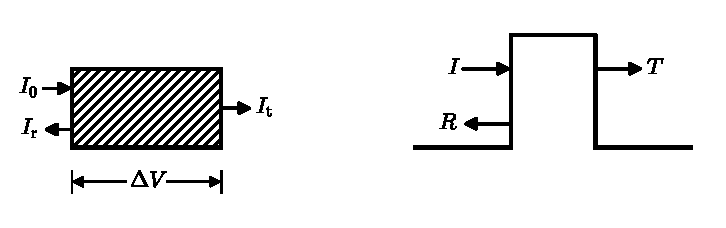
\includegraphics[width=9cm]{fig12-6.pdf}\\[0.3em]
{\small (a) 无序样品的透射与反射电流\qquad\qquad (b) 一维无序样品的模拟势垒}\\[0.2em]
{\small 图 12.6}
\end{minipage}
\end{center}

我们将采用文献[22]所给出的简易方法推导一维系统的兰多尔公式.根据图12.6(a)，设电流 $I_{0}$ 从左侧进入一维样品，而 $I_{\mathrm{r}}=RI_{0}$ 为离开样品左侧的反射电流，在右侧的 $I_{\mathrm{t}}=TI_{0}$ 代表流过一维无序样品的透射电流.由于理想的一维系统其横截面往往小到可以忽略的程度，实际流经样品的电流也将非常小，因此在一维系统中真正有意义的物理量是电流密度j.在固体物理学中，对于d维系统（特别是低于三维的系统）的横截面习惯用 $A_{d}=L^{d-1}$（L为d维超立方体的长度）表示，当 $d=1$ 时即使 $L\rightarrow0$ 也将得到一维横截面 $A_{1}=1$.换句话说，在一维系统中的电流I就是电流密度j，人们往往将一维系统中的j直接称为电流I.因此，我们可以将固体物理学中的 $j=nev_{\mathrm{F}}$ 公式（其中：n是电子浓度，$v_{\mathrm{F}}$ 是费密速度，e是电子电荷）直接用于描述一维系统中的电流I的数值.

考虑到在样品左侧理想导体中的电子浓度 $n_{0}$ 应当包括入射电流 $I_{0}$ 和反射电流 $I_{\mathrm{r}}$ 中的所有电子，并利用入射和反射电流的数值和 $\left(I_{0}+I_{\mathrm{r}}\right)$ 表示为
\begin{equation}
  n_{0}=\frac{\left(I_{0}+I_{\mathrm{r}}\right)}{ev_{\mathrm{F}}}
\end{equation}
在样品右侧的电子浓度 $n_{\mathrm{t}}$ 可根据 $I_{\mathrm{t}}=j_{\mathrm{t}}=n_{\mathrm{t}}ev_{\mathrm{F}}$ 求得
\begin{equation}
  n_{\mathrm{t}}=\frac{I_{\mathrm{t}}}{ev_{\mathrm{F}}}
\end{equation}
因此在无序样品两侧理想导线之间的电子浓度差为
\begin{equation}
  \Delta n=n_{0}-n_{\mathrm{t}}=\frac{\left(I_{0}+I_{\mathrm{r}}-I_{\mathrm{t}}\right)}{ev_{\mathrm{F}}}
  =\frac{2RI_{0}}{ev_{\mathrm{F}}}
\end{equation}
其中R为反射系数，显然浓度差 $\Delta n$ 导致反射电流 $I_{\mathrm{r}}$ 的存在.此外，在上式中还利用了
\begin{equation}
  I_{\mathrm{t}}=TI_{0},\qquad I_{\mathrm{r}}=RI_{0}
\end{equation}
以及粒子流守恒条件 $T+R=1$.正是由于样品两侧存在电位差 $\Delta V$，使电子在两侧的浓度差 $\Delta n$ 保持不变，形成恒定的反射电流 $I_{\mathrm{r}}$.另一方面，确定的 $\Delta V$ 将维持 $I_{0}$ 不变，同时又维持了恒定的透射电流 $I_{\mathrm{t}}=TI_{0}$.$\Delta n$ 与 $\Delta V$ 的关系可以利用样品两侧理想导体中费密面上的电密度 $N\left(E_{\mathrm{F}}\right)$ 求出
\begin{equation}
  \Delta n=2N\left(E_{\mathrm{F}}\right)e\Delta V
\end{equation}
其中因子2来源于自旋简并，$N\left(E_{\mathrm{F}}\right)$ 代表费密能级 $E_{\mathrm{F}}$ 处的电子态密度
\begin{equation}
  N\left(E\right)=\frac{\mathrm{d}n\left(p\right)}{\mathrm{d}E}
  =\left[\frac{\mathrm{d}n\left(p\right)}{\mathrm{d}p}\right]\left(\frac{\mathrm{d}p}{\mathrm{d}E}\right)
\end{equation}
由于 $n\left(p\right)=\left(p/\pi\hbar\right)$ 代表一维系统中在动量p以内的状态数，而 $E\left(p\right)\equiv\left(p^{2}/2m\right)$，以及 $p=mv$，可求出 $\left[\mathrm{d}n\left(p\right)/\mathrm{d}p\right]=\left(1/\pi\hbar\right)$ 和 $\left(\mathrm{d}p/\mathrm{d}E\right)=1/v$.因此
\begin{equation}
  N\left(E_{\mathrm{F}}\right)=\left(1/\pi\hbar v_{\mathrm{F}}\right)
\end{equation}
代入 $\Delta n$ 公式(12.7.8)，求出
\begin{equation}
  \Delta V=\frac{\pi\hbar v_{\mathrm{F}}}{2e}\Delta n
\end{equation}
若再将公式(12.7.6)代入上式右边，可得到 $\Delta V=\left(\pi\hbar/e^{2}\right)RI_{0}$.最后，利用 $I_{\mathrm{t}}=TI_{0}$，即可求出一维无序系统的电导公式(12.7.1)
\begin{equation*}
  G\equiv\frac{I_{\mathrm{t}}}{\Delta V}=\left(\frac{e^{2}}{\pi\hbar}\right)\frac{T}{R}
\end{equation*}
此即著名的一维兰多尔电导公式，它是一个适用于描述弹性散射的普遍公式.由于弹性散射就是势散射，它总可以用一个模拟的势垒以及相应的透射系数T和R来表示传导过程.但应注意，当公式推广用于尺寸为L的一维样品时，必须要求L小于非弹性散射的平均距离.20世纪80年代以来，兰多尔公式已普遍应用无序系统，特别是讨论弱定域化问题.近年来，由于实验技术的发展，人们已能制备样品尺寸小于非弹性散射平均间距的介观器件，给兰多尔公式提供了更广阔的应用天地，并已成为研究介观体系的一个普遍公式.

上述兰多尔公式只考虑了在两端连接导线的单个能带中费密能级附近的电子透射与反射，称为单通道的兰多尔公式.对于高维系统，由于连接导线在垂直方向受到尺寸的限制，将产生横向的能级分裂，使样品两端理想导体中的电子分布在横向能级 $E_{n}\ \left(n=1,2,3,\cdots\right)$ 不相同的子能带之中
\begin{equation}
  E_{n}\left(k\right)=E_{n}+\frac{\hbar^{2}k^{2}}{2m}
\end{equation}
其中每一个 $E_{n}$ 相当于一个一维子能带的带边能.由于相邻 $E_{n}$ 的能级间距随横向尺寸减小而增大，对于理想的一维导体，将因其横向尺寸小到可以忽略的程度而使能级间距（例如 $\Delta E_{12}=E_{2}-E_{1}$）趋向无穷大.这时只需要考虑一个子带中的电子散射，此即一维系统为单通道问题的物理原因.显然，将兰多尔公式推广到二维和三维系统时，必须考虑电子从多个子能带出发对样品中势垒的复杂散射问题，这就是多通道情形.有关多通道的兰多尔公式可参阅文献[23].

\subsection*{2. 一维无序系统的平均电阻计算}

首先考虑含有两个杂质散射中心的系统.当应用兰多尔公式处理这一问题时，可将此系统看作两个势垒，其间由常数势隔开某一距离，如图12.7所示\textsuperscript{[24]}.我们的任务是要求出电子波在双势垒间经多次透射和反射后的透射系数 $T_{12}$ 与两个势垒的透射和反射系数 $\left(T_{1},R_{1}\right)$ 和 $\left(T_{2},R_{2}\right)$ 之间的解析关系.一维无序系统的特征可以看作是由一组具有相同 $\left(T_{1},R_{1}\right)$ 和 $\left(T_{2},R_{2}\right)$，但势垒间距不等的双势垒构成的系综.经正确选择无规变量作系综平均后，才能求得一维无序系统中平均电阻随样品尺寸L的变化关系.

\begin{center}
\begin{minipage}{9cm}
\centering
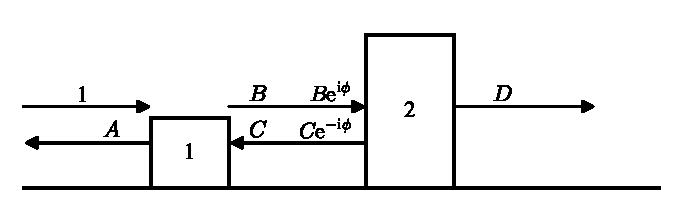
\includegraphics[width=9cm]{fig12-7.pdf}\\{\small 图 12.7\quad 一维无序系统中的双势垒}
\end{minipage}
\end{center}

设入射电子波的振幅为1，经双势垒的多重散射后的总透射与反射波幅分别用D和A表示，而B与C则描述在势垒1右侧的总出射和入射波幅，其中A、B、C和D都是复量.参考图12.7可知，在两势垒之间为常数势场，电子将以平面波 $\mathrm{e}^{\mathrm{i}\left(kx-\omega t\right)}$ 形式自由传播一定距离，必然使1与2两个垫垒内侧的电子之间存在一定的相位差 $\phi$.因此，在图中将势垒2左侧的入射和反射波幅写成 $B\mathrm{e}^{\mathrm{i}\phi}$ 与 $C\mathrm{e}^{-\mathrm{i}\phi}$.现在可以利用 $n=1,2$ 两势垒本身的透射概率幅 $t_{n}$（$T_{n}=|t_{n}|^{2}$——透射系数）和反射概率幅 $r_{n}$ 及反向的反射概率幅 $r_{n}'$（$R_{n}=|r_{n}|^{2}=|r_{n}'|^{2}$——反射系数）写出A、B、C、D所满足的散射方程组
\begin{subequations}
\begin{equation}
  A=r_{1}+Ct_{1}
\end{equation}
\begin{equation}
  B=t_{1}+Cr_{1}'
\end{equation}
\begin{equation}
  C\mathrm{e}^{-\mathrm{i}\phi}=B\mathrm{e}^{\mathrm{i}\phi}r_{2}
\end{equation}
\begin{equation}
  D=B\mathrm{e}^{\mathrm{i}\phi}t_{2}
\end{equation}
\end{subequations}
从上式中(b)、(c)、(d)等方程中消去B和C，求得通过双势垒的透射概率幅 $t_{12}$ 为
\begin{equation}
  t_{12}\equiv D=\frac{\mathrm{e}^{\mathrm{i}\phi}t_{1}t_{2}}
  {1-\mathrm{e}^{\mathrm{i}2\phi}r_{1}'r_{2}}
\end{equation}
因此，双势垒的透射系数
\begin{equation}
  T_{12}=|t_{12}|^{2}=|t_{1}|^{2}
  \frac{1}{|1-\mathrm{e}^{\mathrm{i}2\phi}r_{1}'r_{2}|^{2}}\,|t_{2}|^{2}
\end{equation}
考虑到 $T_{n}=|t_{n}|^{2}$，$r_{1}'=|r_{1}|\mathrm{e}^{-\mathrm{i}\varphi_{1}}=\sqrt{R_{1}}\,\mathrm{e}^{-\mathrm{i}\varphi_{1}}$，$r_{2}=|r_{2}|\mathrm{e}^{\mathrm{i}\varphi_{2}}=\sqrt{R_{2}}\,\mathrm{e}^{\mathrm{i}\varphi_{2}}$，并定义
\begin{equation}
  \theta\equiv 2\phi+\left(\varphi_{2}-\varphi_{1}\right)
\end{equation}
其中 $\phi$ 随1与2势垒的间距变化，这时可将透射系数表示为更简单的形式
\begin{equation}
  T_{12}=\frac{T_{1}T_{2}}{1+R_{1}R_{2}-2\sqrt{R_{1}R_{2}}\cos\theta}
\end{equation}
双势垒的反射系数 $R_{12}$，可利用 $R_{12}+T_{12}=1$ 从 $T_{12}$ 直接求得
\begin{equation}
  R_{12}=\frac{R_{1}+R_{2}-2\sqrt{R_{1}R_{2}}\cos\theta}
  {1+R_{1}R_{2}-2\sqrt{R_{1}R_{2}}\cos\theta}
\end{equation}
最后可将双势垒系统的反射与透射系数比写成
\begin{equation}
  S_{12}=\frac{R_{12}}{T_{12}}
  =\frac{R_{1}+R_{2}-2\sqrt{R_{1}R_{2}}\cos\theta}{T_{1}T_{2}}
  =\frac{1}{T_{12}}-1
\end{equation}
由于在 $\theta$ 因子中还含有两势垒间的相位差 $\phi$，它是一个随势垒间距变化的量，而一维无序系统的主要特征是两个散射中心的间距可随意变化，没有平移对称性.特别是在弱势散射情况，由于杂质的平均间距远大于费密波长，这时 $\phi$ 可取0到 $2\pi$ 间的任一个 $\phi$ 值.对于不同间距的双势垒系统所构成的系综，在0到 $2\pi$ 之间出现任意 $\phi$ 值的概率应当是均等的.因此，我们可以认为 $\theta$ 也以相等的概率出现在0到 $2\pi$ 之间的任意 $\theta$ 角上.安德逊等人正是根据这一特征，计算了函数
\begin{equation}
  f\left(S_{12}\right)=\ln\left(1+S_{12}\right)
  =\ln\left(1+\frac{R_{12}}{T_{12}}\right)=-\ln T_{12}
\end{equation}
的角平均.首先他们计算了 $\ln T_{12}$ 的 $\theta$ 角平均
\begin{equation*}
  \langle\ln T_{12}\rangle=\langle\ln T_{1}\rangle+\langle\ln T_{2}\rangle
  -\left\langle\ln\left(1+R_{1}R_{2}-2\sqrt{R_{1}R_{2}}\cos\theta\right)\right\rangle
\end{equation*}
并令 $a=1+R_{1}R_{2}$ 和 $b=-2\sqrt{R_{1}R_{2}}$，求得上式右边最后一项等于零
\begin{equation}
\begin{aligned}
  \left\langle\ln\left(a+b\cos\theta\right)\right\rangle
  &=\frac{1}{2\pi}\int_{0}^{2\pi}\mathrm{d}\theta\ln\left(a+b\cos\theta\right)\\
  &=\frac{1}{2\pi}\Bigl\{\int_{0}^{\pi}\mathrm{d}\theta\ln\left(a+b\cos\theta\right)\\
  &\qquad-\int_{0}^{\pi}\mathrm{d}\theta\ln\left(a-b\cos\theta\right)\Bigr\}\\
  &=\ln\frac{1}{2}\left[a+\sqrt{a^{2}-b^{2}}\right]
  -\ln\frac{1}{2}\left[a+\sqrt{a^{2}-b^{2}}\right]\\
  &=0
\end{aligned}
\end{equation}
由此求得 $\langle\ln T_{12}\rangle=\langle\ln T_{1}\rangle+\langle\ln T_{2}\rangle$，这是一维无序系统的一个重要特征.若将 $T_{1}$ 与 $T_{2}$ 分别看作是由长度为 $L_{1}$ 和 $L_{2}$ 的两段一维无序样品的透射系数 $T\left(L_{1}\right)$ 和 $T\left(L_{2}\right)$，相应的方程可用反射与透射系数比 $S=R/T$ 表示为
\begin{equation}
  \left\langle\ln\left[1+S\left(L_{1}+L_{2}\right)\right]\right\rangle
  =\left\langle\ln\left[1+S\left(L_{1}\right)\right]\right\rangle
  +\left\langle\ln\left[1+S\left(L_{2}\right)\right]\right\rangle
\end{equation}
这是描述一维无序系统S的对数函数 $f\left(S\right)=\ln\left[1+S\left(L\right)\right]$ 之平均值随样品尺寸改变（即标度变化）的一个重要方程.显然，满足这个方程的解必然是
\begin{equation}
  \langle f\rangle=\left\langle\ln\left[1+S\left(L\right)\right]\right\rangle=\gamma L
\end{equation}
因此，一段长度为L的一维无序样品的 $f=\ln\left[1+S\left(L\right)\right]$ 函数的平均值是L的线性增长函数.安德逊等人还仔细地分析了f函数相对于平均值的均方偏差 $\Delta^{2}\left(L\right)=\langle\left(f-\langle f\rangle\right)^{2}\rangle=\langle f^{2}\rangle-\langle f\rangle^{2}$，并指出在L很大时也具有 $\Delta^{2}\left(L\right)\propto L$ 的线性增长特征\textsuperscript{[20]}.显然，当L很大时f的相对偏差 $\left[\Delta\left(L\right)/\langle f\rangle\right]$ 正比于 $L^{-\frac{1}{2}}$，在 $L\rightarrow\infty$ 时，它趋向于零，满足概率论的中心极限定理（即大数定律），可以用f相对于其平均值 $\langle f\rangle$ 偏离很小的高斯分布描述.因此，作为初级近似，可以认为 $\langle f\rangle$ 就是一维无序系统的实际 $\ln\left[1+S\left(L\right)\right]$ 函数，并求得实际的反射与透射系数比为
\begin{equation}
  S\left(L\right)=\frac{1-T\left(L\right)}{T\left(L\right)}
  =\left(\mathrm{e}^{2\alpha L}-1\right)
\end{equation}
其中设 $\gamma=2\alpha$.由于 $S\left(L\right)$ 实际上代表以 $\left(\pi\hbar/e^{2}\right)$ 为单位的量纲为1的电阻，其倒数定义以 $\left(e^{2}/\pi\hbar\right)$ 为单位的量纲为1的电导，根据式(12.7.1)与式(12.7.24)有
\begin{equation}
  g\left(L\right)\equiv G\left(L\right)/\left(\frac{e^{2}}{\pi\hbar}\right)
  =\frac{T\left(L\right)}{1-T\left(L\right)}
  =\left(\mathrm{e}^{2\alpha L}-1\right)^{-1}
\end{equation}
由此立刻求出一维无序系统的实际透射概率（即透射系数）为
\begin{equation}
  T\left(L\right)=\mathrm{e}^{-2\alpha L}
\end{equation}
因此，在一维无序系统中，经L距离的透射后，电子波的概率幅减小了 $\mathrm{e}^{-\alpha L}$ 倍，从而十分清楚地告诉我们对传导起主要作用的费密能级 $\left(E_{\mathrm{F}}\right)$ 上的电子波函数是指数衰减型 $\exp\left(-|\boldsymbol{r}-\boldsymbol{R}|/\lambda\right)$ 的定域态，其中 $\lambda=\alpha^{-1}$ 代表定域化长度.不言而喻，系统中的其它电子，因其能级 $E<E_{\mathrm{F}}$，也必然处于定域化状态.换句话说，一维无序系统中的所有电子均处于定域化状态.

\subsection*{3. 用量纲为1的电导 $g(L)$ 描述定域化}

由于在“2”中，利用正确的无规平均方法，求得了一维无序系统中量纲为1的电导 $g\left(L\right)$ 随样品长度L变化的公式(12.7.25)，我们可以换一个观点直接从可测物理量 $g\left(L\right)$ 的标度（即L变化）特征来描述一维无序系统的定域化.用标度变化的观点讲：当L增大时，如果量纲为1的电导 $g\left(L\right)$ 随之单调地减小，并在 $L\rightarrow\infty$ 时有 $g\left(L\right)\rightarrow0$ 的特点时，系统处于定域态.反之，当 $g\left(L\right)$ 随L增大单调地上升时，系统处于扩展态.这是一种区分扩展态与定域态的简单而有效的方案，它适用于任意的d维 $\left(d=1,2,3\right)$ 系统.

对于一维无序系统，从式(12.7.25)可以看出，存在 $g\left(L\right)\ll1$ 和 $g\left(L\right)\gg1$ 两个极限
\begin{equation}
  g\left(L\right)=\left(\mathrm{e}^{2L/\lambda}-1\right)^{-1}
  =\begin{cases}
    \dfrac{\lambda}{2L} & \left[g\left(L\right)\gg1\ \text{或}\ L\ll\lambda\right]\\[0.8em]
    \mathrm{e}^{-2L/\lambda} & \left[g\left(L\right)\ll1\ \text{或}\ L\gg\lambda\right]
  \end{cases}
\end{equation}
显然，$g\left(L\right)$ 随着样品尺寸L增大，从 $g\left(L\right)\gg1$ 极限单调地减小，并连续地过渡到另一极限 $g\left(L\right)\ll1$.当 $L\rightarrow\infty$ 时，$g\left(L\right)\rightarrow0$，这说明一维无序系统中电子处于定域态，其中 $g\left(L\right)\gg1$ 极限对应于 $\alpha L\ll1$（$\alpha=\lambda^{-1}$）的弱定域化情形，而另一极限 $\alpha L\gg1$ 则代表强定域化.弱定域化即弱散射情形，后者可用半经典的玻耳兹曼输运理论描述，主要的结论是，对于任意的d维系统，电流密度j与电场强度E之间满足欧姆定律 $j=\sigma E$，其中导电率 $\sigma=\left(ne^{2}l/mv_{\mathrm{F}}\right)$，$v_{\mathrm{F}}$ 为费密速度，l是平均自由程，n代表电子浓度.显然，在弱散射极限，$\sigma$ 是一个与系统尺寸L无关的强度量.用于边长为L的d维立方体，当样品两端存在电位差V时，沿某方向的总电流应为 $I=jL^{d-1}$，其中 $L^{d-1}$ 是垂直流动方向的横截面积.电位差V可认为是L长度样品中均匀电场E所产生，有 $V=EL$ 关系.因此，d维立方体的电导
\begin{equation}
  G\equiv I/V=\left(j/E\right)L^{d-2}
\end{equation}
当欧姆定律 $j=\sigma E$ 成立时，d维系统的电导可表示为
\begin{equation}
  G\left(L\right)=\sigma L^{d-2}
\end{equation}
其中 $\sigma$ 为一个与L无关的常数.对应的量纲为1的电导在弱散射极限为
\begin{equation}
  g\left(L\right)=\left(\frac{\pi\hbar}{e^{2}}\right)\sigma L^{d-2}
\end{equation}
不难看出，满足欧姆定律的电导在 $d=1$ 时正比于 $L^{-1}$，与弱定域化情形（$\alpha L\ll1$ 时）的 $g\left(L\right)=\dfrac{\lambda}{2}L^{-1}$ 相似，比例系数均与L无关.在文献中往往将式(12.7.30)称为扩展态（或金属）极限.以后（见§8）读者将明白，上式仅在 $d>2$ 情形才具有 $g\left(L\right)$ 随L上升而增大的扩展态特征，对于 $d\leqslant2$ 的低维系统（特别是 $d=1$ 时），它仅属于弱定域化情形.但是，$g\left(L\right)\gg1$ 特征却是普遍成立的.因此，确切地说，式(12.7.30)只是d维系统在 $g\left(L\right)\gg1$ 时的渐近表示式.至于另一个极限 $g\left(L\right)\ll1$，若将式(12.7.27)推广到d维系统，可以表示为 $g\left(L\right)=g_{d}\exp\left(-2L/\lambda\right)$，其中 $g_{d}$ 是一个数量级为1，且与L无关的常数.在明白了这些基础知识以后，才能推广讨论在任意维度d时无序系统中定域化的标度理论.历史也正如此，兰多尔早在1970年就导出了描述一维系统定域化的正确公式(12.7.27)，只是他所用的平均方法欠妥当.本节“2”中所介绍的是1980年安德逊等人的改进无规平均方法，但结果仍然与兰多尔一致.

\section{定域化的标度理论}

1979年，亚伯拉罕（E.Abrahams）和安德逊等四人\textsuperscript{[14]}首先提出了无序系统的标度理论.他们采用长度为L的d维块体的量纲为1的电导 $g\left(L\right)$ 作为描述定域化特征的唯一标度参量，并仿照重整化群的标度理论，对不同维度无序体系的定域化特征作出了一系列新的预言，包括：与一维相似，在二维无序体系中也不存在扩展态，所有的态都是定域化的.仅在三维无序体系中，才可能既有定域态又有扩展态，并且从扩展态变为定域态的M-I（金属-绝缘体）转变是连续的，而不存在莫特所预言的最小金属电导率 $\sigma_{\mathrm{min}}$.这些新成果的出现，使人们对安德逊定域化的认识进入了更深的层次，也为无序系统的定域化研究打开了新的窗口.

本节主要介绍描述定域化的标度参量 $g\left(L\right)$，亚伯拉罕等人的标度假定及其对 $d=1,2,3$ 维无序体系的应用.最后指出标度理论所存在的问题.

\subsection*{1. 描述定域化的标度参量 $g(L)$}

在本章§5讨论安德逊无序模型时，已经证明：三维无序系统的特征主要由定域化参数 $\delta\equiv\left(W/2ZV\right)$ 的大小决定，其中Z为近邻格点的配位数，W代表格点（原子）上电子能级的无规分布宽度（即对角无序的量度），而V则描述电子在近邻格点（原子）之间跃迁的交叠能量积分，又称原子间跃迁的共振能量.因此，在原子尺度上看，量纲为1的比值 $\left(V/W\right)$ 正比于定域化参数 $\delta$ 的倒数 $\left(\delta^{-1}\right)$.在标度理论中，人们需要引入一个随系统尺寸L变化的相应量纲为1的参量来描述定域化的标度特征.为此，可将上述讨论作推广，考虑由边长为L的d维立方块体 $\left(L^{d}\right)$ 构成的大样品，设 $V_{L}$ 代表两相邻d维块体间电子跃迁的共振能量，它是原子间跃迁共振能V的块体推广.当 $L\gg l,a$ 时（其中l为电子的平均自由程，a为平均原子间距），还可以引入块体 $L^{d}$ 内电子能级的平均间距 $\Delta_{L}$ 描述无序的强度，因为它正比于电子能级的无规分布的宽度W.$\Delta_{L}$ 可以利用L块体中单位体积内的费密能级态密度 $N_{L}\left(E_{\mathrm{F}}\right)$ 近似决定
\begin{equation}
  \Delta_{L}=\left[N\left(E_{\mathrm{F}}\right)L^{d}\right]^{-1}\sim W
\end{equation}
这是一个随块体尺寸L变化的量.至于近邻块体间的跃迁共振能量 $V_{L}$，当 $L\gg l$ 并略去非弹性散射条件下，可以模拟为电子在近邻块体间的势垒隧穿问题.根据量子力学的不确定关系，$V_{L}=\left(\pi\hbar/\tau_{L}\right)$，可将 $V_{L}$ 改用 $\tau_{L}$ 描述，这里 $\tau_{L}$ 代表电子在近邻块体间通过隧穿转移所需的时间.当两相邻块体间存在电位差 $\widetilde{V}$ 时，将有 $\left[N_{L}\left(E_{\mathrm{F}}\right)L^{d}e\widetilde{V}\right]$ 个状态上的电子从势垒的一侧流向另一侧.相应的，电流可表示为 $I=\left[e^{2}N_{L}\left(E_{\mathrm{F}}\right)L^{d}/\tau_{L}\right]\widetilde{V}$，因此L块体的电导
\begin{equation}
\begin{aligned}
  G\left(L\right)&=e^{2}N_{L}\left(E_{\mathrm{F}}\right)L^{d}/\tau_{L}\\
  &=\frac{e^{2}}{\pi\hbar}\left(V_{L}/\Delta_{L}\right)
\end{aligned}
\end{equation}
其中利用了式(12.8.1)和不确定关系 $V_{L}\tau_{L}=\pi\hbar$.根据上节中讨论，块体的电导 $g\left(L\right)$ 恰好等于块体的量纲为1的比值 $\left(V_{L}/\Delta_{L}\right)$
\begin{equation}
  g\left(L\right)\equiv G\left(L\right)/\left(\frac{e^{2}}{\pi\hbar}\right)=\left(\frac{V_{L}}{\Delta_{L}}\right)
\end{equation}
在文献中 $\left(V_{L}/\Delta_{L}\right)$ 称为索勒斯（Thouless）比，它就是安德逊无序模型中参数 $\delta^{-1}$ 的有限尺寸推广.式(12.8.3)表明：人们可以用可测量的物理量 $g\left(L\right)$ 描述d维块体中定域化特征随标度L的改变，而且是描述无序系统定域化特征的唯一标度参量.因此，当 $L\rightarrow\infty$ 时有 $g\left(L\right)\rightarrow0$，就表示系统处于定域态.反之，当 $L\rightarrow\infty$ 时若 $g\left(L\right)\rightarrow\infty$，则说明系统为扩展态.换句话说，只需要讨论量纲为1的电导 $g\left(L\right)$ 的标度特征，就可以对d维无序系统倒底是处于定域态、扩展态，还是两者兼有等重要问题作出明确的判断.这就是亚伯拉罕等人建立定域化标度理论的思路.

\subsection*{2. 标度假定和标度方程}

亚伯拉罕等人的标度理论是建立在d维电导 $g\left(L\right)$ 在半经典的弱散射极限 $\left[g\left(L\right)\gg1\right]$ 和强定域化极限 $\left[g\left(L\right)\ll1\right]$ 的下列已知特征的一个外插理论.根据式(12.7.30)及其后的讨论，已知
\begin{equation}
  g\left(L\right)=
  \begin{cases}
    \left(\dfrac{\pi\hbar}{e^{2}}\right)\sigma L^{d-2} & \left[g\left(L\right)\gg1\right]\\[0.8em]
    g_{d}\,\mathrm{e}^{-2\alpha L} & \left[g\left(L\right)\ll1\right]
  \end{cases}
\end{equation}
其中 $\sigma$ 为与L无关的常数，$g_{d}$ 是数量级为1的常数.为了进一步讨论 $g\left(L\right)$ 如何随样品尺寸L变化，他们仿照重整化群理论，利用 $\ln g\left(L\right)$ 对 $\ln L$ 的导数描述 $g\left(L\right)$ 的变化，并利用式(12.8.4)写出在上述两种极限情形的已知关系：
\begin{equation}
  \beta=\frac{\mathrm{d}\ln g\left(L\right)}{\mathrm{d}\ln L}
  =\begin{cases}
    d-2 & \left[g\left(L\right)\gg1\right]\\
    \ln\left(g\left(L\right)/g_{d}\right)=-2\alpha L & \left[g\left(L\right)\ll1\right]
  \end{cases}
\end{equation}
其中d表示体系的维度.定域化标度理论是假定在两极限之间对数导数 $\beta$ 随L的变化仅仅通过 $g\left(L\right)$ 的改变表示，即假定 $\beta$ 仅仅是 $g\left(L\right)$ 的函数.$\beta$ 满足下列标度方程：
\begin{equation}
  \beta\left[g\left(L\right)\right]=\frac{\mathrm{d}\ln g\left(L\right)}{\mathrm{d}\ln L}
  =\frac{L}{g\left(L\right)}\,\frac{\mathrm{d}g\left(L\right)}{\mathrm{d}L}
\end{equation}
并且进一步猜测 $\beta$--$\ln g\left(L\right)$ 曲线在两已知极限 $g\left(L\right)\gg1$ 与 $g\left(L\right)\ll1$ 之间连续单调的变化.根据上述假定求解标度方程，可得知 $d=1,2,3$ 维无序体系的标度特征，如图12.8所示.我们将在“3”中对此作进一步的讨论.至于标度方程式(12.8.6)的引入相当于在将样品尺寸扩大b倍时 $\left(L\rightarrow L'=bL\right)$，假定新尺寸的电导 $g\left(bL\right)$ 仅由前一尺寸L时的电导 $g\left(L\right)$ 决定，此即假定
\begin{equation}
  g\left(bL\right)=f\left[g\left(L\right),\,b\right]
\end{equation}

\begin{center}
\begin{minipage}{8cm}
\centering
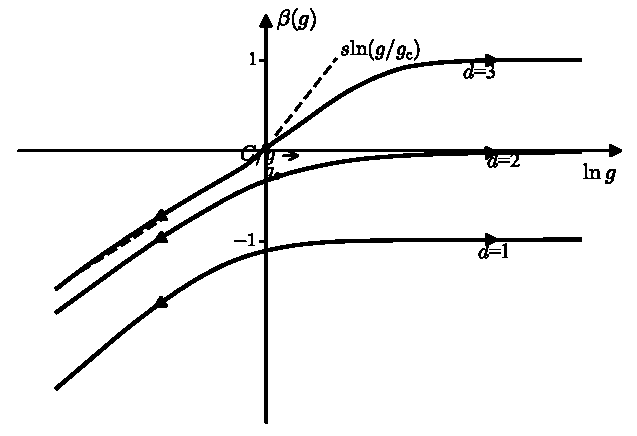
\includegraphics[width=8cm]{fig12-8.pdf}\\{\small 图 12.8\quad $d=1$、2、3 维体系的 $\beta$--$\ln g$ 曲线}
\end{minipage}
\end{center}

这是f是一个与系统具体微观结构无关的普适函数.若令 $b=1+\varepsilon$，其中 $\varepsilon\rightarrow0$，相当于对系统作无限小的标度变换，这时可立刻从上式导出标度方程
\begin{equation}
\begin{aligned}
  \frac{\mathrm{d}\ln g\left(L\right)}{\mathrm{d}\ln\left(L\right)}
  &=\frac{1}{g\left(L\right)}\lim_{\varepsilon\to0}
  \frac{f\left[g\left(L\right),\,1+\varepsilon\right]-f\left[g\left(L\right),\,1\right]}{\varepsilon}\\
  &=\frac{1}{g\left(L\right)}
  \frac{\partial f\left[g\left(L\right),\,b\right]}{\partial b}\bigg|_{b=1}
  \equiv\beta\left[g\left(L\right)\right]
\end{aligned}
\end{equation}
此即式(12.8.6)的标度假定.标度方程的简便之处在于可根据 $\beta$ 取正或负值来判断当标度L改变时电导 $g\left(L\right)$ 是上升或下降，从而区分扩展态与定域态.

\subsection*{3. 标度方程的应用}

现在应用标度方程式(12.8.6)和在两极限的已知 $\beta$ 结果具体讨论一维，三维和二维无序体系的定域化特征.为了简单起见，先讨论 $g\left(L\right)$ 为已知的一维无序系统.

（i）一维系统

这时 $\beta$ 在两个极限均取负值
\begin{equation}
  \beta=
  \begin{cases}
    -1 & \left[g\left(L\right)\gg1,\ g\left(L\right)\sim L^{-1}\right]\\
    -2\alpha L & \left[g\left(L\right)\ll1,\ g\left(L\right)\sim\mathrm{e}^{-2\alpha L}\right]
  \end{cases}
\end{equation}
根据标度假定所作的连续光滑 $\beta$ 曲线如图12.8中 $d=1$ 曲线所示，其中的箭头表示L增大时的流动方向.显然，当L增大时，不仅 $\beta$ 从 $\left(-1\right)$ 降为 $\left(-\infty\right)$，相应的 $g\left(L\right)$ 也单调减小，并在 $L\rightarrow\infty$ 时按指数规律 $\mathrm{e}^{-2\alpha L}$ 趋向于零，说明在一维无序系统中电子处于定域态，而不存在扩展态.由于在上节中我们已经导出了一维无序系统中电导随标度L的变化为 $g\left(L\right)=\left(\mathrm{e}^{2\alpha L}-1\right)^{-1}$，在这里可以直接求出
\begin{equation}
  \beta\left[g\left(L\right)\right]=\frac{\mathrm{d}\ln g\left(L\right)}{\mathrm{d}\ln L}
  =-\left[1+g\left(L\right)\right]\ln\left[1+g^{-1}\left(L\right)\right]
\end{equation}
这就证明了 $\beta$ 的确仅仅是 $g\left(L\right)$ 的函数，并且当L增大时 $g\left(L\right)$ 总是单调的减小，$\beta$ 从 $\left(-1\right)$ 到 $\left(-\infty\right)$ 的流动是单向的，不存在扩展态，这些都与亚伯拉罕等人的标度理论所预言的结果一致.不仅如此，上式还能给出 $\beta\rightarrow\left(-1\right)$ 时 $\beta$ 函数的渐近式
\begin{equation}
  \beta\left[g\left(L\right)\right]=-1-\frac{1}{2g\left(L\right)}
  \qquad\left[g\left(L\right)\gg1\right]
\end{equation}
其中 $-\dfrac{1}{2g\left(L\right)}$ 为，在 $g\left(L\right)\gg1$ 区域内，$\beta$ 函数的修正项.这一结果可推广用于d维系统，并写成
\begin{equation}
  \beta\left[g\left(L\right)\right]=d-2-\frac{C}{g\left(L\right)}
  \qquad\left[g\left(L\right)\gg1\right]
\end{equation}
上式对于 $d=2$、3维情形是一个有用的渐近式，其中常数 $C>0$.

（ii）三维系统

当 $d=3$ 时，式(12.8.5)给出标度函数 $\beta\left(g\right)$ 在两已知极限分别取正、负值
\begin{equation}
  \beta\left(g\right)=
  \begin{cases}
    +1 & \left[g\left(L\right)\gg1,\ g\left(L\right)\sim\sigma L\right]\\
    -2\alpha L & \left[g\left(L\right)\ll1,\ g\left(L\right)\sim\mathrm{e}^{-2\alpha L}\right]
  \end{cases}
\end{equation}
按照标度假定，连接 $\beta=+1$ 与 $\beta=-\infty$（$L\rightarrow\infty$ 时，$\beta\rightarrow-\infty$）两已知极限间的 $\beta\left(g\right)$ 连续曲线必与横轴 $\ln g$ 相交，交点在 $g=g_{\mathrm{c}}$ 处，它是标度函数 $\beta\left(g\right)$ 的零点，满足 $\beta\left(g_{\mathrm{c}}\right)=0$，如图12.8中 $d=3$ 曲线所示.由于 $\beta=0$ 即 $\left(\mathrm{d}g/\mathrm{d}L\right)=0$，因此在 $\beta\left(g_{\mathrm{c}}\right)=0$ 点的电导 $g_{\mathrm{c}}$ 将不随L变化，包括取 $L\rightarrow\infty$ 时该点的电导仍等于 $g_{\mathrm{c}}$，在这个意义上 $g_{\mathrm{c}}$ 被称为不动点.这是一个不稳定的不动点，因为从不动点 $\beta\left(g_{\mathrm{c}}\right)=0$ 的上方 $\left(g>g_{\mathrm{c}}\right)$ 或下方 $\left(g<g_{\mathrm{c}}\right)$ 作标度变换（使L增大）均将导致系统的状态代表点 $g\left(L\right)$ 离开不动点 $g_{\mathrm{c}}$.例如，当 $g>g_{\mathrm{c}}$ 时标度函数 $\beta>0$，由于 $\left(\mathrm{d}g/\mathrm{d}L\right)>0$，$g\left(L\right)$ 必随标度L的增大而升高，表现为状态代表点 $g\left(L\right)$ 将沿 $\beta$ 曲线向上流动，并远离不动点 $g_{\mathrm{c}}$，最后在 $L\rightarrow\infty$ 时到达 $\beta=+1$ 和 $g\rightarrow\infty$ 点，这时系统的 $g\left(L\right)\sim\sigma L$，其中 $\sigma$ 与L无关，称为标准的金属极限.显然，在不动点 $\beta\left(g_{\mathrm{c}}\right)=0$ 的上方 $\beta>0$ 区域内电子具有扩展态特征，被称为三维无序系统的金属（或扩展）区.反之，在不动点的下方从 $g<g_{\mathrm{c}}$ 点出发作标度变换，由于 $\beta<0$，$\left(\mathrm{d}g/\mathrm{d}L\right)<0$，状态代表点 $g\left(L\right)$ 将随L增大而减小，它也将远离不动点但沿 $\beta$ 曲线向下流动，最后到达强定域化极限，并在 $L\rightarrow\infty$ 时按指数规律下降到 $g\rightarrow0$ 和 $\beta\rightarrow-\infty$ 点.因此，在不稳定的不动点下方 $\beta<0$ 区域内，系统具有定域态特征，可称为绝缘（或定域）区.总之，在三维无序系统中既有扩展态，又有定域态，并在不动点 $g_{\mathrm{c}}$ 处发生扩展态与定域态之间的转变，称为金属-绝缘体（M-I）转变.由于 $g>g_{\mathrm{c}}$ 时系统为导体，而 $g<g_{\mathrm{c}}$ 时为绝缘体，不动点 $g_{\mathrm{c}}$ 应与本章§5中的迁移率边界相对应.当无序系统中电子的费密能级 $E_{\mathrm{F}}$ 与迁移率边界的能量 $E_{\mathrm{c}}$ 相等时，到达不动点 $g_{\mathrm{c}}$ 并发生M-I转变.

为了得知在迁移率边界 $E_{\mathrm{c}}$ 附近系统电导率随电子能量E的变化特征，考虑在扩展区靠近不动点 $g_{\mathrm{c}}$ 的一个点 $g_{0}>g_{\mathrm{c}}$，其中 $g_{0}\left(E\right)\equiv g\left(E_{\mathrm{F}},L_{0}\right)$，$L_{0}$ 代表某一微观尺度，而E在 $E_{\mathrm{F}}$ 附近.当 $E_{\mathrm{F}}$ 等于 $E_{\mathrm{c}}$ 时，到达不动点 $g_{\mathrm{c}}=g_{0}\left(E_{\mathrm{c}}\right)\equiv g\left(E_{\mathrm{c}},L_{0}\right)$.对于 $g\left(L\right)$ 十分接近 $g_{\mathrm{c}}$ 情形，根据线性近似，可用标度函数 $\beta$ 在 $g_{\mathrm{c}}$ 点的斜率s表示
\begin{equation}
  \beta\left(g\right)=s\left[g\left(L\right)-g_{\mathrm{c}}\right]
\end{equation}
为了符合金属极限的渐近关系，当 $g\rightarrow\infty$ 时 $\beta\rightarrow1$，人们往往将上式推广为\textsuperscript{[25]}
\begin{equation}
  \beta\left(g\right)=\frac{s\left[g\left(L\right)-g_{\mathrm{c}}\right]}
  {1+s\left[g\left(L\right)-g_{\mathrm{c}}\right]}
\end{equation}
将上式代入标度函数 $\beta$ 的定义式(12.8.6)，并从某一微观尺度 $L_{0}$ $\left[g\left(L_{0}\right)\right.$ 十分接近 $\left.g_{\mathrm{c}}\right]$ 积分到足够大的宏观尺度L（$\beta$ 接近1），可求得下列关系式
\begin{equation}
  \left[\left(\frac{g\left(L_{0}\right)-g_{\mathrm{c}}}{g\left(L\right)-g_{\mathrm{c}}}\right)
  \left(\frac{g\left(L\right)}{g\left(L_{0}\right)}\right)\right]^{\nu}
  \frac{g\left(L_{0}\right)}{g\left(L\right)}=\frac{L_{0}}{L}
\end{equation}
其中 $\nu\equiv\left(sg_{\mathrm{c}}\right)^{-1}$.考虑到在宏观尺度L时 $\beta$ 接近经典的金属极限，等式
\begin{equation}
  \sigma=\left(\frac{e^{2}}{\pi\hbar}\right)\frac{g\left(L\right)}{L}
\end{equation}
成立，并且电导率 $\sigma$ 与L无关，它只是电子能量E（在 $E_{\mathrm{F}}$ 附近）的函数.再考虑到 $g\left(L\right)\gg g_{\mathrm{c}}$ 和 $g\left(L_{0}\right)$ 十分接近 $g_{\mathrm{c}}$，式(12.8.16)可写为
\begin{equation}
  \frac{g\left(L\right)}{L}\approx\frac{g_{\mathrm{c}}}{L_{0}}
  \left(\frac{g_{0}-g_{\mathrm{c}}}{g_{\mathrm{c}}}\right)^{\nu}
\end{equation}
代入式(12.8.17)得到
\begin{equation}
  \sigma\sim\left(g_{0}-g_{\mathrm{c}}\right)^{\nu}
\end{equation}
其中指数 $\nu$ 的数值计算结果大致为1.5.再注意到 $g_{0}\equiv g\left(E,L_{0}\right)$ 和 $g_{\mathrm{c}}\equiv g\left(E_{\mathrm{c}},L_{0}\right)$，当 $g_{0}$ 十分接近不动点 $g_{\mathrm{c}}$ 时，电子能量E必然靠近迁移率边界 $E_{\mathrm{c}}$，有 $\left(g_{0}-g_{\mathrm{c}}\right)\sim\left(E-E_{\mathrm{c}}\right)$ 关系，这时可将电导率表示为
\begin{equation}
  \sigma=\sigma_{\mathrm{c}}\left(E-E_{\mathrm{c}}\right)^{\nu}
\end{equation}
其中 $\sigma_{\mathrm{c}}$ 为一常数.式(12.8.19)与式(12.8.20)表明：改变电子的能量使 $E\rightarrow E_{\mathrm{c}}$ 和 $g_{0}$ 过渡为 $g_{\mathrm{c}}$，三维系统的电导率将连续下降为零，在迁移率边界 $E_{\mathrm{c}}$ 处M-I转变是连续的，不存在莫特所预言的最小金属电导率 $\sigma_{\mathrm{min}}$，这是定域化标度理论的另一个重要结论.

（iii）二维系统

当 $d=2$ 时，应计入弱散射区的修正公式(12.8.12)，并将式(12.8.5)改写为
\begin{equation}
  \beta=
  \begin{cases}
    -C/g\left(L\right) & \left[g\left(L\right)\gg1,\ g\sim\sigma\right]\\
    -2\alpha L & \left[g\left(L\right)\ll1,\ g\sim\mathrm{e}^{-2\alpha L}\right]
  \end{cases}
\end{equation}
上式表明在 $\infty>g\left(L\right)\geqslant0$ 区域内二维系的标度函数 $\beta\left(g\right)$ 总小于零.这时，在 $\beta$ 很小的区域内，对渐近式
\begin{equation*}
  \mathrm{d}\ln g\left(L\right)/\mathrm{d}\ln L=-C/g\left(L\right)
\end{equation*}
作积分，积分的下限取某一微观尺度 $L_{0}$，上限 $L\ll\alpha^{-1}$（其中 $\alpha^{-1}=\lambda$）仍限于弱散射区，得到
\begin{equation*}
  g\left(L\right)=g_{0}-C\ln\left(L/L_{0}\right)
\end{equation*}
其中 $g_{0}$ 为尺度 $L_{0}$ 时的电导.显然，当标度L增大时，状态的代表点从 $g_{0}$ 沿 $d=2$ 曲线向下方流动，与强定域化区内的流向一致，整个二维曲线只有一种向下的流动方向.因此二维体系没有真正的扩展态，它与一维无序体系相似，所有的状态都是定域化的.另一方面，当 $g_{0}$ 很大时，$\beta$ 值接近于零，增大标度时电导的下降十分缓慢，表明在弱定域化区内二维样品仍可能有良好的导电性.

\subsection*{4. 存在的问题}

定域化的标度理论，包括：一维与二维无序体系的基态是绝缘相，只有在三维无序体系中才可能既有绝缘又有金属相，还存在金属-绝缘体转变，并且这个M-I转变是连续的等特征均已得到了实验的支持.近二十年来这些结论已成为一种信念被人们所接受.但是，标度理论只是建立在 $g\gg1$ 和 $g\ll1$ 极限间具有单调外插行为基础上的简单理论，它的主要问题是忽略了电子之间的相互作用.随后的理论研究表明，电子间库仑作用对于一维和三维系统的结论并无本质性的改变，简单标度理论的主要结果仍然适用于一维和三维无序体系.但是对于二维系统，由于它介于一维与三维之间，实际上相当复杂，在理论研究上也一直存在着争议.值得一提的是，早在20世纪80年代中期前苏联学者\textsuperscript{[26]}曾经指出，来自电子间相互作用的量子修正在一定条件下可使二维系统的电阻率随温度降低而减小，从而导致二维系统在低温时可能形成金属相，只是由于当时缺乏实验证据，未能受到重视.近年来由于半导工艺和技术的进步，已经能够在相当宽的范围内调节二维电子系统的浓度.克拉夫钦科（Kravchenko）等人\textsuperscript{[27]}在高质量二维样品中研究了无外磁场时的低温电导特性，他们发现在低浓度下，将实验结果内插到 $T=0$ K时电阻趋向无穷大，表明这时二维系统的基态仍是绝缘性的，与传统的标度理论一致.但是当二维电子系统的浓度超过某临界值后，电阻将随温度降低而减小，并在 $T=0$ K时趋向于零，又表现出金属性，这是与传统的信念相反的新实验结果.换句话说，实验证实了在无外磁场时二维无序体系与三维情形相似，既存在绝缘相又存在金属相，并且改变电子浓度可导致二维系统中出现从绝缘体向金属的转变，这是一个令人吃惊的结果.1997年多布洛舍甫杰维奇（Dobrosavljevic）与亚伯拉罕等人\textsuperscript{[28]}在计入电子间库仑关联的影响后，又提出了一个新的标度理论，其基本点是认为并无任何基本原理要求 $\beta\left(g\right)$ 曲线必须是单调函数以及在 $g\left(L\right)\gg1$ 时二维系统中 $\beta$ 必须为负，因此可以假定在 $g\left(L\right)\gg1$ 时
\begin{equation}
  \beta\left(g\right)=\left(d-2\right)+A/g^{\alpha}+\cdots
  \qquad\left(A>0\right)
\end{equation}
用于代替式(12.8.12)，这时所有的 $d\geqslant2$ 系统 $\beta$ 函数均可能在某些有限的 $g=g_{\mathrm{c}}$ 点上改变符号，导致三维与二维系统中都可能出现M-I转变.对于二维系统可取 $\alpha=1$，其标度行为如图12.9所示.由图可知，在二维无序体系中也可能存在两种基态：其一是具有无限大电阻的绝缘性基态，另一个则是具有无限大电导的金属基态.如何严格证明二维系统的非单调标度行为确实如图12.9所示是当前凝聚态理论研究的一个重要问题.此外，无外磁时二维无序电子系统中是否存在金属基态也还需要更多的实验证据.

\begin{center}
\begin{minipage}{10cm}
\centering
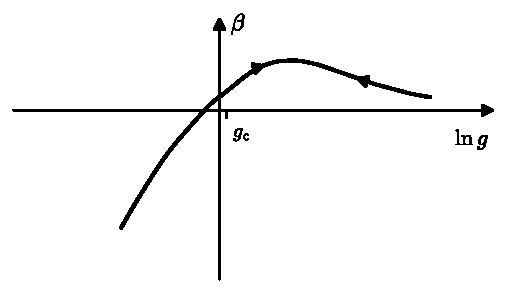
\includegraphics[width=7cm]{fig12-9.pdf}\\{\small 图 12.9\quad 二维系统中 $\beta$--$\ln g$ 曲线的非单调行为}
\end{minipage}
\end{center}

\begin{canKao}
\begin{enumerate}[label={[\arabic*]}, leftmargin=2.2em, itemsep=0pt]
\item Yonezawa F. The Structure and Properties of Matter. Ed. Matsubara T. Berlin: Springer Press, 1982. Chap 11
\item Soven P. Phys Rev, 1967, 156: 809
\item Taylor D W. Phys Rev, 1967, 156: 1017
\item 李正中等. Phys Rev，1994，B50：11332；Phys Rev，1991，B43：12906；Phys Lett，1988，A131：466
\item 许望，李正中. J Phys，1988，C21：4083；J Phys，1990，CM2：109；Solid State Commun，1991，80：943
\item Mott N F. Adv Phys, 1967, 16: 49
\item 李雅达（Lee P W）. 物理通讯，1980，4：46
\item Anderson P W. Phys Rev, 1958, 109: 1492
\item Thouless D J. J Phys, 1970, C3: 1559
\item Ziman J M. J Phys., 1960, C2: 1230; Model of Disorder. Cambridge Univ Press, 1979. Chap 9
\item Licciardello D C, Economon E N. Phys Rev, 1975, B11: 3 697
\item Mott N F et al. Proc Roy Soc (London), 1975, A345: 169
\item 韩汝琦. 自然杂志，1981，3：256
\item Abrahans E, Anderson P W, Licciardello D C, Ramakrisbnan T V. Phys Rev Lett, 1979, 42: 673
\item Sarker S, Domany E. Phys Rev, 1981, B23: 6 018
\item 阎守胜. 固体物理基础. 北京大学出版社，2000
\item Mott N F. J Non Crystal Solids, 1968, 1: 1
\item Mott N F, Twose W D. Adv Phys, 1961, 10: 107
\item Abrikosov A A et al. Adv Phys, 1978, 24: 147
\item Anderson P W et al. Phys Rev, 1980, B22: 3 519
\item Landauer R. Phil Mag, 1970, 21: 863
\item Erdos P et al. Adv Phys, 1982, 31: 65
\item 田光善. 介观物理. 见：阎守胜，甘子钊主编. 北京大学出版社，1995.25
\item Imry Y. Introduction to Mesoscopic Physics. Oxford: Oxford Univ Press, 1997. Chap 5
\item Isihara A. Electron Liqids. New York: Springer, 1992
\item Finkel'stein A M. Z Phys, 1984, B56: 189
\item Kravchenko S V et al. Phys Rev, 1994, 50: 8 039; 1995, 51: 7 038
\item Dobrosavljevic V, Abrahams E et al. Phys Rev Lett, 1997, 42: 673
\end{enumerate}
\end{canKao}
